\documentclass[a4paper,12pt,twoside]{report}
\usepackage[utf8]{inputenc}
\usepackage{hyperref}
\usepackage{graphicx}
\usepackage{geometry}
\usepackage{color}
\usepackage{fancyhdr}
\usepackage{tikz}
\usetikzlibrary{patterns}
\usepackage{titlesec}
\usepackage{lmodern}
\usepackage{setspace}
\usepackage{framed}
\usepackage{lipsum}
\usepackage{indentfirst}
\usepackage{amsmath,amssymb,enumerate,pgf}
\usepackage{physics}
\usepackage{amsthm}
\usepackage{caption}
\usepackage{subcaption}


\usepackage[
backend=biber,
style=alphabetic,
sorting=ynt
]{biblatex}
\addbibresource{sample.bib}

\DefineBibliographyStrings{english}{%
  bibliography = {References},
}

\newcommand{\mtn}{\mathbb{N}}
\newcommand{\mtns}{\mathbb{N}^*}
\newcommand{\mtz}{\mathbb{Z}}
\newcommand{\mtr}{\mathbb{R}}
\newcommand{\mtk}{\mathbb{K}}
\newcommand{\mtq}{\mathbb{Q}}
\newcommand{\mtc}{\mathbb{C}}
\newcommand{\mch}{\mathcal{H}}
\newcommand{\mcp}{\mathcal{P}}
\newcommand{\mcb}{\mathcal{B}}
\newcommand{\mcl}{\mathcal{L}}
\newcommand{\mcm}{\mathcal{M}}
\newcommand{\mcc}{\mathcal{C}}
\newcommand{\mcmn}{\mathcal{M}}
\newcommand{\mcmnr}{\mathcal{M}_n(\mtr)}
\newcommand{\mcmnk}{\mathcal{M}_n(\mtk)}
\newcommand{\mcsn}{\mathcal{S}_n}
\newcommand{\mcs}{\mathcal{S}}
\newcommand{\mcd}{\mathcal{D}}
\newcommand{\dif}{\mathrm{d}}
\newcommand{\mcsns}{\mathcal{S}_n^{++}}
\newcommand{\glnk}{GL_n(\mtk)}
\newcommand{\mnr}{\mathcal{M}_n(\mtr)}
\DeclareMathOperator{\ch}{ch}
\DeclareMathOperator{\sh}{sh}
\DeclareMathOperator{\vect}{vect}
\DeclareMathOperator{\card}{card}
\DeclareMathOperator{\comat}{comat}
\DeclareMathOperator{\imv}{Im}
\DeclareMathOperator{\rang}{rg}
\DeclareMathOperator{\Fr}{Fr}
\DeclareMathOperator{\diam}{diam}
\DeclareMathOperator{\supp}{supp}
\DeclareMathOperator{\mat}{mat}
\newcommand{\veps}{\varepsilon}
\newcommand{\mcu}{\mathcal{U}}
\newcommand{\mcun}{\mcu_n}
\newcommand{\dis}{\displaystyle}
\newcommand{\croouv}{[\![}
\newcommand{\crofer}{]\!]}
\newcommand{\rab}{\mathcal{R}(a,b)}
\newcommand{\pss}[2]{\langle #1,#2\rangle}
\DeclareMathOperator{\sign}{sign}

\newtheorem{theorem}{Theorem}[section]
\newtheorem{corollary}{Corollary}[theorem]
\newtheorem{lemma}[theorem]{Lemma}


\newcommand{\ReportTitle}{Contribution to the development of the Psydac}
\author{Arasu Candassamy}

\geometry{top=2cm, bottom=2cm, left=1.5cm, right=1.5cm}

\pagestyle{fancy}
\fancyhf{} 
\fancyhead[CE]{\rightmark}   
\fancyhead[CO]{\ReportTitle} 
\fancyfoot[C]{\textbf{Arasu Candassamy} / Max-Planck-Institute Für Plasmaphysik \\
\textcolor{red}{\textbf{Non-confidential report and Can be published on the Internet}}}
\fancyfoot[R]{\thepage}
\renewcommand{\footrulewidth}{0.5pt}

\fancypagestyle{plain}{
    \fancyhf{} 
    \fancyhead[CE]{\rightmark}   
    \fancyhead[CO]{\ReportTitle} 
    \fancyfoot[C]{\textbf{Arasu Candassamy} / Max-Planck-Institute Für Plasmaphysik \\
    \textcolor{red}{\textbf{Rapport Non-confidentiel et publiable sur Internet}}}
    \fancyfoot[R]{\thepage}
    \renewcommand{\footrulewidth}{0.5pt}
}

\fancypagestyle{test}{
    \fancyhf{} 
    \fancyhead[CE]{}   
    \fancyhead[CO]{} 
    \fancyfoot[C]{\textbf{Arasu Candassamy} / Max-Planck-Institute Für Plasmaphysik \\
    \textcolor{red}{\textbf{Rapport Non-confidentiel et publiable sur Internet}}}
    \fancyfoot[R]{\thepage}
    \renewcommand{\footrulewidth}{0.5pt}
}

% Permet à \leftmark et \rightmark de fonctionner correctement
\renewcommand{\chaptermark}[1]{\markright{#1}}
\renewcommand{\sectionmark}[1]{\markright{#1}{}}


\begin{document}
\thispagestyle{empty}

% Logos
\begin{minipage}{0.6\textwidth}
    
\includegraphics[width=5cm]{logoENSTA.jpg} 
\end{minipage}
\hfill
\begin{minipage}{0.6\textwidth}
    
\includegraphics[width=5cm]{logoMPI.png}
\end{minipage}

\vspace{2cm}

\begin{center}
    {\LARGE \textbf{Projet de Recherche (PRe)}}
    
    \vspace{0.5cm}
    \textbf{Spécialité : Mathématiques Appliquées} \\
    \textbf{Année scolaire : 2024-2025}
    
    \vspace{2cm}
    
    {\Huge \textcolor{gray}{Contribution to the development of the Psydac and Struphy finite element libraries.}} \\
    
    \vspace{1.5cm}
        
    \begin{framed}
        \centering
        \textcolor{red}{\textbf{Rapport Non-confidentiel et publiable sur Internet}} 
    \end{framed}
\end{center}


\begin{minipage}[t]{0.5\textwidth}
	\begin{flushleft} 
    \textbf{Auteur} : Arasu Candassamy \\
    \vspace{1cm}
	\textbf{Tuteur ENSTA :}\\
	\textsc{Sonia Fliss}\\
	\href{mailto:sonia.fliss@ensta.fr}{sonia.fliss@ensta.fr}
	\end{flushleft}
\end{minipage}
~
\begin{minipage}[t]{0.4\textwidth}
	\begin{flushright} 
    \textbf{Promotion} : 2026 \\
    \vspace{1cm}
	\textbf{Tuteur Organisme d'accueil :}\\
	\textsc{Martin Campos-Pinto}\\
	\href{mailto:martin.campos-pinto@ipp.mpg.de}{martin.campos-pinto@ipp.mpg.de}\\
	\end{flushright}
\end{minipage} \\

\vspace{1cm}

\begin{center}
    \textbf{Stage effectué} du 26/05/2025 au 22/08/2025\\
\textbf{Nom de l’organisme d’accueil :} Max-Planck-Institute Für Plasmaphysik\\
\textbf{Adresse :} Boltzmannstrasse 2, 85748 Garching bei München
\end{center}


\newpage\null

\newpage
\section*{Abstract}
\addcontentsline{toc}{chapter}{Abstract}

\lipsum[1-2]

\vspace{1cm}

\underline{Keywords}:

\vspace{1cm}

\section*{Résumé}

\lipsum[1-2]

\vspace{1cm}

\underline{Mots-clés}:

\newpage\null

\newpage

\section*{Acknowledgement}
\addcontentsline{toc}{chapter}{Acknowledgement}
\lipsum[1-2]


\newpage
\tableofcontents
\thispagestyle{test}


\newpage
\chapter{Introduction}

The Max-Planck Institute for Plasma Physics (IPP), located in Garching and Greifswald, is a renowned research institute in Plasma physics and Nuclear fusion. Founded under the Max-Planck Society in 1960, this institute has a long tradition of scientific excellence and innovation. The Department of Numerical Methods for Plasma Physics (NMPP), where my internship took place, plays a crucial role in developing advanced simulation techniques to understand and predict the behavior of plasmas in complex environments (in tokamaks or stelerators). \\

The Finite Element Method (FEM) is a widely used numerical technique for solving Partial Differential Equations (PDEs). It is particularly well-suited for addressing plasma physics problems due to its ability to handle complex geometries and varied boundary conditions. FEM allows for the discretization of a continuous domain into a set of finite elements, thereby facilitating the numerical resolution of equations governing the physical phenomena under study. \\

In the context of electromagnetism, the Finite Element Exterior Calculus (FEEC) formulation is a powerful approach for solving Maxwell's equations. This method is particularly suitable for problems involving electromagnetic fields, as it preserves certain topological and physical properties of the original equations. FEEC provides a powerfull framework for plasma simulation, where electromagnetic interactions play a central role. \\

Psydac is an integrated development environment (IDE) specifically designed for simulation and data analysis in plasma physics. It offers a range of tools to facilitate the implementation of numerical methods, including FEM and FEEC frameworks. Psydac enables researchers to develop complex models, simulate them, and analyze results efficiently and intuitively. Psydac also stands out as an isogeometric analysis library, an approach that integrates geometric modeling and numerical analysis within a unified framework. Isogeometric analysis allows simulations to be performed directly on the geometric models used for design, eliminating the need to convert CAD models into traditional meshes for simulations. This provides increased accuracy and better integration between design and analysis, reducing errors and improving the efficiency of the simulation process. Using Psydac, researchers can leverage these capabilities to develop more accurate models and perform more reliable analyses, which is particularly advantageous in the complex field of plasma physics. \\

This internship report describes my experience and contributions within the NMPP Department at the IPP. Psydac should be able to solve any PDEs but it hasn't been tested on equations from solid mechanics. Then, during this internship, I have explored the linear elasticity problem, its simulation using Psydac and its running on Supercomputer Raven.

\chapter{Linear Elasticity}

\section{Physical Model and Strong Formulation}
The following presentation of the context of work and physical background comes from \cite{gould_introduction_2013} and \cite{ern_theory_2004}. \\
Let's denote by $\Omega \subset \mtr^3$ a deformable medium characterized by $\lambda$ and $\mu$ Lamé's coefficient ($\lambda, \mu > 0$). $\Omega$ is a bounded open domain with lipschitzian boundary. $\lambda$ is called Lamé's first coefficient, $\mu$ is the shear modulus. These coefficient are related to the Young modulus and Poisson coefficient of the medium. The deformable medium is under an external load $\vec f : \Omega \rightarrow \mtr^3$. Then, we are looking for $\vec u : \Omega \rightarrow \mtr^3$ the displacement field, when the equilibrium is reached. 

The material verifies the following equilibrium condition : 
\begin{equation}
\label{eq:equilibrium}
    \div \boldsymbol{\sigma} (\vec u) + \vec f = \vec 0 \text{ in } \Omega,
\end{equation}
where $\boldsymbol{\sigma} (\vec u)$ is the Cauchy Stress Tensor, defined by $\boldsymbol{\sigma} (\vec u) = C : \boldsymbol{\varepsilon} (\vec u)$. $C$ is the fourth-order stiffness tensor and $$\boldsymbol{\varepsilon} (\vec u) := \frac{1}{2}(\grad \vec u + (\grad \vec u)^T)$$ is the strain tensor. In the context of linear elascity, the relation between $\boldsymbol{\varepsilon} (\vec u)$ and $\boldsymbol{\sigma} (\vec u)$ is simpler : 

\begin{equation}
\label{eq:hooklaw}
    \boldsymbol{\sigma} (\vec u) = \lambda \Tr(\boldsymbol{\varepsilon}) I_3 + 2\mu \boldsymbol \varepsilon = \lambda (\div \vec u) I_3 + \mu (\grad \vec u + (\grad \vec u)^T) \text{ in } \Omega.
\end{equation}

For boundary conditions, there are two types of boundary conditions : Dirichlet conditions on the displacement field $\vec u$ and Traction conditions on the Cauchy Stress Tensor $\boldsymbol \sigma (\vec u)$. 


\begin{figure}[!h]
	\centering
	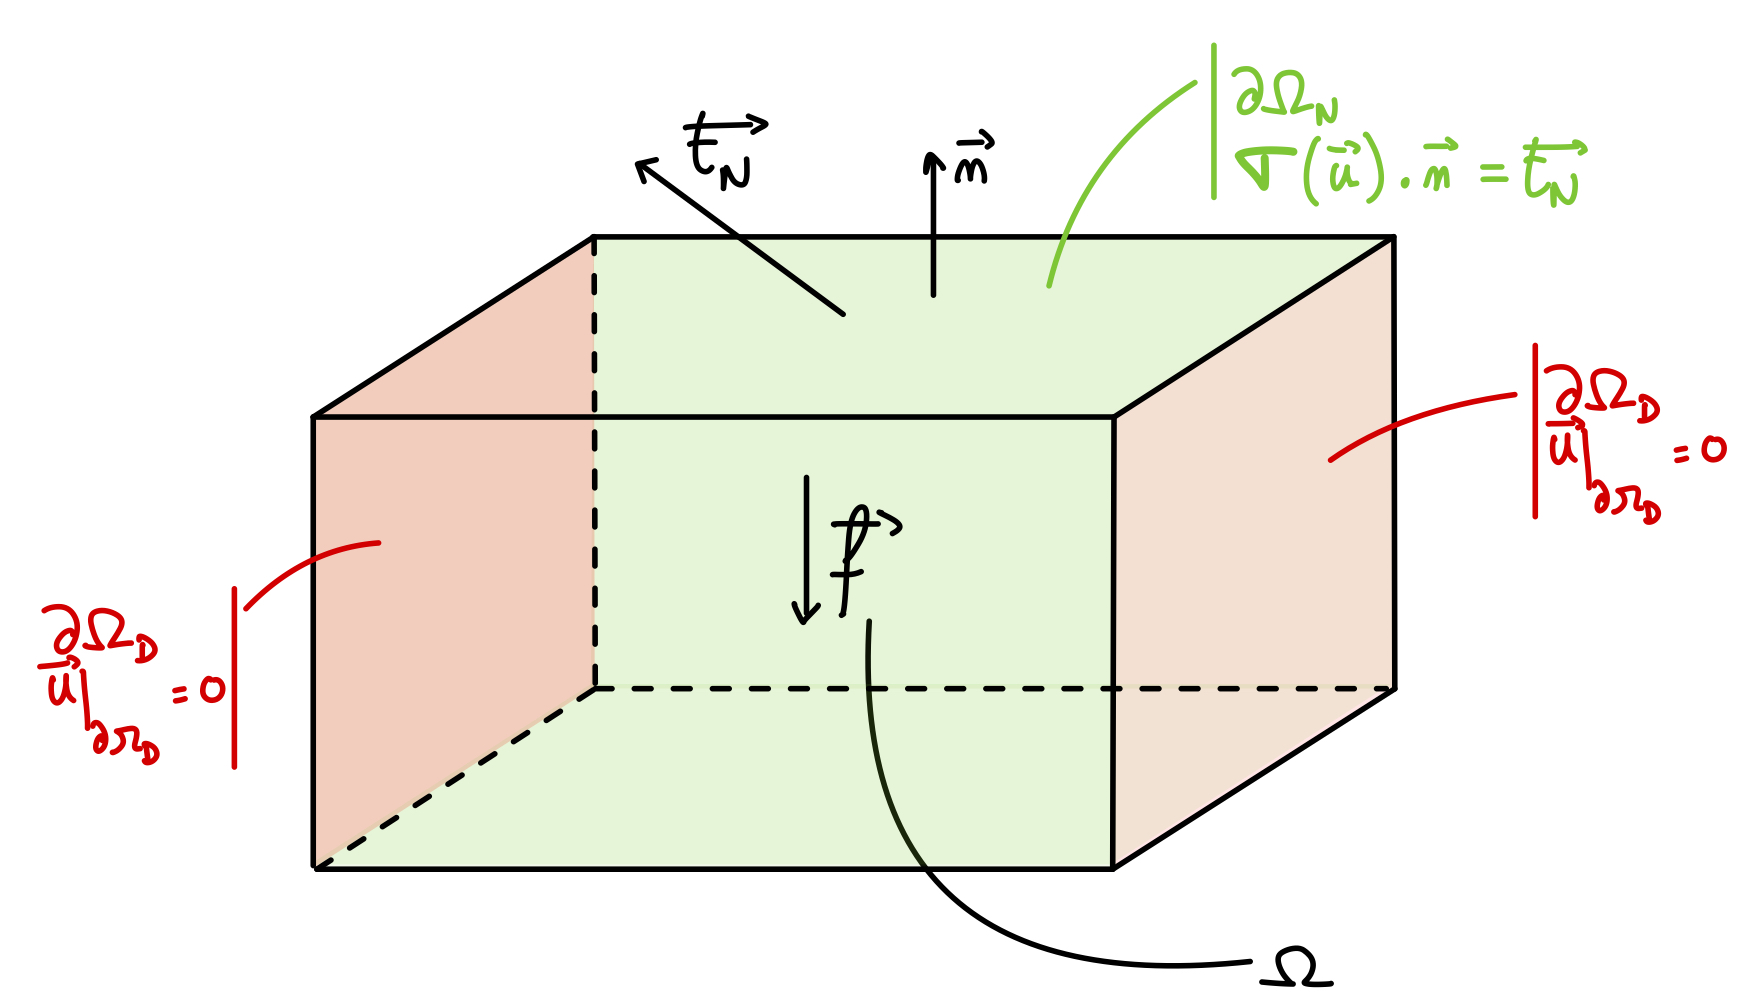
\includegraphics[width=0.61\linewidth]{omega_domain}
	\caption{Representation of a domain $\Omega$}
	\label{fig:omegadomain}
\end{figure}

Let's decompose $\partial \Omega$ as $\partial \Omega_D$ and $\partial \Omega_N$ such that $\partial \Omega_D \cup \partial \Omega_N = \partial \Omega$, $\partial \Omega_D \cap \partial \Omega_N = \emptyset$. Let's denote by $\vec t_N : \partial \Omega_N \rightarrow \mtr^3$ the normal traction force and $\vec n$ the normal vector of $\partial \Omega$ outside-oriented. We can consider the boundary displacement on $\partial \Omega_D$ as equal to $\vec 0$. 

In case of non-homogenous boundary conditions $\vec g : \partial \Omega_D \rightarrow \mtr^3$, we can solve the problem for $\vec u - \vec g$ by modifying the source term. Then, the solution of linear elasticity problem should verify :
$$
\left\{ \begin{array}{ll}
\vec u = \vec 0 & \partial \Omega_D \\
\boldsymbol{\sigma} (\vec u) \cdot \vec n = \vec t_N & \partial \Omega_N
\end{array} \right.
$$

Physically, $\vec f$ is a "volume force" on $\Omega$ and $\vec t_N$ is a "surface force". 
The strong formulation of this problem is : \\
For a given $\vec f \in \boldsymbol L^2(\Omega)$, $\vec t_N \in \boldsymbol L^2(\partial \Omega_N)$, find $\vec u \in \boldsymbol H^1(\Omega)$ such that : 

\begin{equation}
\label{eq:strong_form}
\left \{
\begin{aligned}
    & - \div \boldsymbol{\sigma} (\vec u) = \vec f & \text{ in } & \Omega \hspace{1cm} \text{(Equilibrium)}\\
    & \boldsymbol{\sigma} (\vec u) = \lambda (\div \vec u) I_3 + \mu (\grad \vec u + (\grad \vec u)^T) & \text{ in }& \Omega \hspace{1cm} \text{(Hook's law)} \\
    & \vec u = \vec 0 & \text{ in } &\partial \Omega_D \\
    & \boldsymbol{\sigma} (\vec u) \cdot \vec n = \vec t_N & \text{ in }& \partial \Omega_N
\end{aligned}
\right.
\end{equation}

where $\boldsymbol L^2(\Omega) = \left(L^2(\Omega) \right)^3, \boldsymbol L^2(\partial \Omega_N) = \left(L^2(\partial \Omega_N) \right)^3, \boldsymbol H^1(\Omega) = \left(H^1(\Omega) \right)^3, $

\section{Pure displacement weak-formulation} \label{sec:Pure displacement weak-formulation}

To derive the weak formulation from \eqref{eq:strong_form}, let's introduce the following functionnal space : $$\boldsymbol H^1_{\vec 0,D}(\Omega) = \left\{ \vec v \in \boldsymbol H^1(\Omega) \Big| \vec v_{|\partial\Omega_D} = \vec 0 \right\},$$
which is a sub-hilbert space of $\boldsymbol H^1(\Omega)$ equipped with the same dot product (as a closed space of a Hilbert space). By taking the scalar product of the equilibrium equation from \eqref{eq:strong_form} with $\vec v \in \left(H^1_{\vec 0,D}(\Omega) \right)^3$ and applying a Green's formula, one gets that :
$$\int_\Omega \boldsymbol{\sigma} (\vec u) : (\grad \vec v) \dif V - \int_{\partial\Omega} \left(\boldsymbol{\sigma} (\vec u).\vec n \right).\vec v \dif S = \int_\Omega \vec f . \vec v \dif V$$

One can remark that with \eqref{eq:hooklaw}, the tensor $\boldsymbol \sigma (\vec u)$ is symetric. It implies that : 
$$\boldsymbol \sigma (\vec u) : \grad \vec v = \boldsymbol \sigma(\vec u) : \boldsymbol \varepsilon (\vec v)$$
Moreover, $\vec v \in \left(H^1_{\vec 0,D}(\Omega) \right)^3$, then $\vec v_{|\partial\Omega_D} = \vec 0$. So the weak formulation can be simplified into : 

\begin{equation}
\label{eq:weakdisplacementform}
\boxed{
\left\{
    \begin{aligned}
    &\text{Find } \vec u \in \boldsymbol H^1_{\vec 0,D}(\Omega) \text{ such that :}\\
    & a(\vec u,\vec v) = l(\vec v) \hspace{0.5cm} \forall \vec v \in \boldsymbol H^1_{\vec 0,D}(\Omega)
    \end{aligned}
\right.
}
\end{equation}

With : 
\begin{equation*}
    \begin{aligned}
        & a : \left\{
        \begin{aligned}
            &\boldsymbol H^1_{\vec 0,D}(\Omega) \times \boldsymbol H^1_{\vec 0,D}(\Omega)  \rightarrow \mtr \\
            &(\vec u,\vec v)  \longmapsto \int_\Omega \boldsymbol \sigma(\vec u) : \boldsymbol \varepsilon (\vec v) \dif V = \int_\Omega \lambda (\div \vec u) (\div \vec v) \dif V+ \int_\Omega 2\mu \boldsymbol \varepsilon(\vec u): \boldsymbol \varepsilon (\vec v)\dif V
        \end{aligned}
        \right. \\[0.3cm]
    & l : \left\{
        \begin{aligned}
            &\boldsymbol H^1_{\vec 0,D}(\Omega) \rightarrow \mtr \\
            &\vec v \longmapsto \int_\Omega \vec f . \vec v \dif V + \int_{\partial\Omega_N} \vec t_N.\vec v \dif S
        \end{aligned}
        \right.
    \end{aligned}
\end{equation*}
In continuum mechanics, \eqref{eq:weakdisplacementform} is called the Principle of Virtual Work. Let's look at the well-posedness of \eqref{eq:weakdisplacementform}. Before starting, let's remind some notations and lemmas. \\

$\norm{.}_{\boldsymbol H^1(\Omega)}$ is defined as : $\forall \vec v \in \boldsymbol H^1(\Omega), \norm{\vec v}_{\boldsymbol H^1(\Omega)} = \left(\sum_{i=1}^3 \norm{v}_{H^1(\Omega)} \right)^{1/2}$. 
\begin{lemma}
\begin{enumerate}
    \item $\displaystyle \forall \vec u \in \boldsymbol H^1(\Omega)$, $$\int_\Omega (\div \vec u)^2 \dif V \leq 3 \norm{\vec u}_{\boldsymbol H^1(\Omega)}^2$$
    \item $\displaystyle \forall \vec u \in \boldsymbol H^1(\Omega)$,$$\boldsymbol \varepsilon(\vec u) : \boldsymbol \varepsilon(\vec u) \leq \grad \vec u : \grad \vec u$$
    Then : $$\int_\Omega \boldsymbol \varepsilon(\vec u) : \boldsymbol \varepsilon(\vec u) \dif\Omega \leq \int_\Omega \grad \vec u : \grad \vec u \dif \Omega \leq \norm{\vec u}_{\boldsymbol H^1(\Omega)}^2$$
\end{enumerate}
\end{lemma}
\begin{proof}
    By calculus, or a detailed version in \cite{cinatl_finite}
\end{proof}

\begin{lemma}
\label{Korn1}
    (First Korn's inequality) \\
    Let $\Omega \subset \mtr^3$ a domain and denotes by $\norm{\boldsymbol \varepsilon(\vec u)}_{\boldsymbol L^2(\Omega)} := \left(\int_\Omega \boldsymbol \varepsilon(\vec u):\boldsymbol \varepsilon(\vec u)\right)^{1/2}$. Then, there exists $C > 0$ such that: $$\forall \vec v \in \boldsymbol H^1_{\vec 0}(\Omega), \hspace{1cm} C\norm{\vec v}_{\boldsymbol H^1(\Omega)} \leq \norm{\boldsymbol \varepsilon(\vec v)}_{\boldsymbol L^2(\Omega)}$$
\end{lemma}
\begin{proof}
    A proof can be found in \cite{brenner_mathematical_2008}
\end{proof}

\begin{lemma}
\label{Korn2}
    (Second Korn's inequality) \\
    Let $\Omega \subset \mtr^3$ a domain. Then, there exists $C > 0$ such that: 
    $$\forall \vec v \in \boldsymbol H^1(\Omega), \hspace{1cm} C\norm{\vec v}_{\boldsymbol H^1(\Omega)} \leq \norm{\boldsymbol \varepsilon(\vec v)}_{\boldsymbol L^2(\Omega)} + \norm{\vec v}_{\boldsymbol L^2(\Omega)}$$
    By Rellich theorem, $\boldsymbol H^1(\Omega)$ is compactly embedded in $\boldsymbol L^2(\Omega)$ as $\Omega$ is a open bounded domain . Then, one can show that there exists $C > 0$ such that:
    $$\forall \vec v \in \boldsymbol H^1(\Omega), \hspace{1cm} C\norm{\vec v}_{\boldsymbol H^1(\Omega)} \leq \norm{\boldsymbol \varepsilon(\vec v)}_{\boldsymbol L^2(\Omega)}$$
\end{lemma}
\begin{proof}
    A proof can be found in \cite{brenner_mathematical_2008}
\end{proof}


\noindent \textbf{Now, we can prove the well-posedness of \eqref{eq:weakdisplacementform} when $\left| \Omega_D \right| > 0$.}
\begin{itemize}
    \item $\left(\boldsymbol H^1_{\vec 0,D}(\Omega), \norm{.}_{\boldsymbol H^1(\Omega)} \right)$ is a Hilbert space.
    \item $a(.,.)$ is a bilinear form on $\boldsymbol H^1_{\vec 0,D}(\Omega) \times \boldsymbol H^1_{\vec 0,D}(\Omega)$ and $l(.)$ a linear form on $\boldsymbol H^1_{\vec 0,D}(\Omega)$.
    \item $l(.)$ is continuous : \begin{equation*}
    \begin{aligned}    
    \forall \vec v \in \boldsymbol H^1_{\vec 0,D}(\Omega), \left|l(\vec v)\right| 
    & \leq \left| \left(\vec f, \vec v \right)_{\boldsymbol L^2(\Omega)} + \left(\vec t_N, \vec v \right)_{\boldsymbol L^2(\partial \Omega_N)} \right| \\
    % & \leq \left| \left(\vec f, \vec v \right)_{\boldsymbol L^2(\Omega)} \right| + \left| \left(\vec t_N, \vec v \right)_{\boldsymbol L^2(\partial \Omega_N)} \right| \\
    % & \leq \norm{\vec f}_{\boldsymbol L^2(\Omega)}\norm{\vec v}_{\boldsymbol L^2(\Omega)} + \norm{\vec t_N}_{\boldsymbol L^2(\partial \Omega_N)}\norm{\vec v}_{\boldsymbol L^2(\partial \Omega_N)} \\
    % & \leq \norm{\vec f}_{\boldsymbol L^2(\Omega)}\norm{\vec v}_{\boldsymbol H^1(\Omega)} + \norm{\vec t_N}_{\boldsymbol L^2(\partial \Omega_N)}\norm{\vec v}_{\boldsymbol L^2(\partial \Omega)} \\
    % & \leq \norm{\vec f}_{\boldsymbol L^2(\Omega)}\norm{\vec v}_{\boldsymbol H^1(\Omega)} + \norm{\gamma_0} \norm{\vec t_N}_{\boldsymbol L^2(\partial \Omega_N)}\norm{\vec v}_{\boldsymbol H^1(\Omega)} \\
    \left|l(\vec v)\right| 
    & \leq \left( \norm{\vec f}_{\boldsymbol L^2(\Omega)} + \norm{\gamma_0} \norm{\vec t_N}_{\boldsymbol L^2(\partial \Omega_N)}\right)\norm{\vec v}_{\boldsymbol H^1(\Omega)}\\
    \end{aligned}
    \end{equation*}
    \item $a(.,.)$ is continuous: 
    \begin{equation*}
        \begin{aligned}
        \forall \vec u, \vec v \in \boldsymbol H^1_{\vec 0,D}(\Omega), \left| a(\vec u, \vec v) \right| 
        & \leq \left| a(\vec u, \vec u) \right|^{1/2} \left| a(\vec v, \vec v) \right|^{1/2} & \text{By Cauchy-Schwarz Inequlity as $a(.,.)$ is} \\
        & & \text{a symetric and positive bilinear form} \\
        \left| a(\vec u, \vec v) \right| & \leq (3\lambda + 2\mu)\norm{\vec u}_{\boldsymbol H^1(\Omega)}\norm{\vec v}_{\boldsymbol H^1(\Omega)}.
        \end{aligned}
    \end{equation*}
    \item $a(.,.)$ is coercive: 
        \begin{itemize}
            \item If $\Omega_D = \Omega$, then $\boldsymbol H^1_{\vec 0,D}(\Omega) = \boldsymbol H^1_{\vec 0}(\Omega)$ and we can apply \textbf{Lemma \ref{Korn1}} : there exists $C > 0$ such that:
            \begin{equation*}
                \begin{aligned}
                    \forall \vec u \in \boldsymbol H^1_{\vec 0,D}(\Omega), \hspace{0.3cm} a(u,u) 
                    &= \int_\Omega \lambda (\div \vec u)^2 \dif V + \int_\Omega 2\mu \boldsymbol \varepsilon(\vec u): \boldsymbol \varepsilon (\vec u)\dif V \\
                    & \geq 2\mu \norm{\boldsymbol \varepsilon(\vec u)}_{\boldsymbol{L}^2(\Omega)} \\
                    a(u,u) & \geq 2\mu C \norm{\vec u}_{\boldsymbol{H}^1(\Omega)}
                \end{aligned}
            \end{equation*}
            \item If $\Omega_D \subsetneq \Omega$, we can now apply \textbf{Lemma \ref{Korn2}} : there exists $C >0$ such that:
            $$\forall \vec u \in \boldsymbol H^1_{\vec 0,D}(\Omega), \hspace{0.3cm}a(u,u) \geq 2\mu C \norm{\vec u}_{\boldsymbol{H}^1(\Omega)}$$
        \end{itemize}
\end{itemize}

Then, by Lax-Milgram theorem, the problem \eqref{eq:weakdisplacementform} is well-posed when $\left| \Omega_D \right| > 0$. \\
When, $\left| \Omega_D \right| = 0$, \eqref{eq:weakdisplacementform} turns into the\textbf{ Pure Traction Problem} : 

\begin{equation}
\label{eq:puretractionproblem}
\boxed{
\left\{
    \begin{aligned}
    &\text{Find } \vec u \in \boldsymbol H^1(\Omega) \text{ such that :}\\
    & a(\vec u,\vec v) = \int_\Omega \vec f . \vec v \dif V + \int_{\partial\Omega} \vec t_N.\vec v \dif S =:l(\vec v) \hspace{0.5cm} \forall \vec v \in \boldsymbol H^1(\Omega)
    \end{aligned}
\right.
}
\end{equation}

This problem isn't really well-posed. Regarding to the Rigid Displacement Field (translations and rotations) $\boldsymbol{\mathcal{R}} = \left\{\vec v \in \boldsymbol H^1(\Omega) \left| \exists x_1, x_2 \in \mtr^3, \vec v(x) = x_1 + x_2 \times x \right. \right\}$, $$\forall \vec v \in \boldsymbol{\mathcal{R}}, \hspace{0.3cm} \div v = 0 \text{ and } \boldsymbol \varepsilon(\vec v) = 0.$$
Then : $$\forall \vec u \in \boldsymbol H^1(\Omega), \forall \vec v \in \boldsymbol{\mathcal{R}},\hspace{0.3cm} a(\vec u, \vec v)= 0.$$
So, the weak formulation \eqref{eq:puretractionproblem} is solvable iff the following compatibility equality holds : $$\forall \vec v \in \boldsymbol{\mathcal{R}}, \hspace{0.3cm}\int_\Omega \vec f . \vec v \dif V + \int_{\partial\Omega} \vec t_N.\vec v \dif S = 0,$$
and in this case, there exists an unique solution $\vec u \in \hat{\boldsymbol H}^1(\Omega) := \left\{\vec v \in \boldsymbol H^1(\Omega) \left| \displaystyle \int_\Omega \vec v \dif V = \int_\Omega  \curl \vec v \dif V = \vec 0 \right. \right\}$ 
In case of \textbf{Pure Traction Problem}, we are looking for a solution modulo a rigid displacement field.
\textit{A more rigorous proof of the equivalence can be found in \cite{brenner_mathematical_2008} and \cite{chen_variational}.}


\section{Numerical simulation using \texttt{PSYDAC} on the Supercomputer Raven}

\texttt{PSYDAC} is high-level programming IDE and very intuitive to use. It is using \texttt{SymPDE} and \texttt{Pyccel}. \texttt{SymPDE} implements in \texttt{Python} abstract objects (Functionnal Space, diffential operators, linear and bilinear forms...). \texttt{Pyccel} is a transpiler, used to convert a \texttt{Python} Code into a \texttt{C} or \texttt{Fortran} code, in order to take advantage from code acceleration and parallelization. The figure \ref{fig:Dependancy_Psydac} summarize the dependancy between \texttt{PSYDAC}, \texttt{SymPDE} and \texttt{Pyccel}. A more detailled presentation of \texttt{PSYDAC} can be found in \cite{guclu_psydac_2022}.
\newpage 

\begin{figure}[!h]
    \centering
    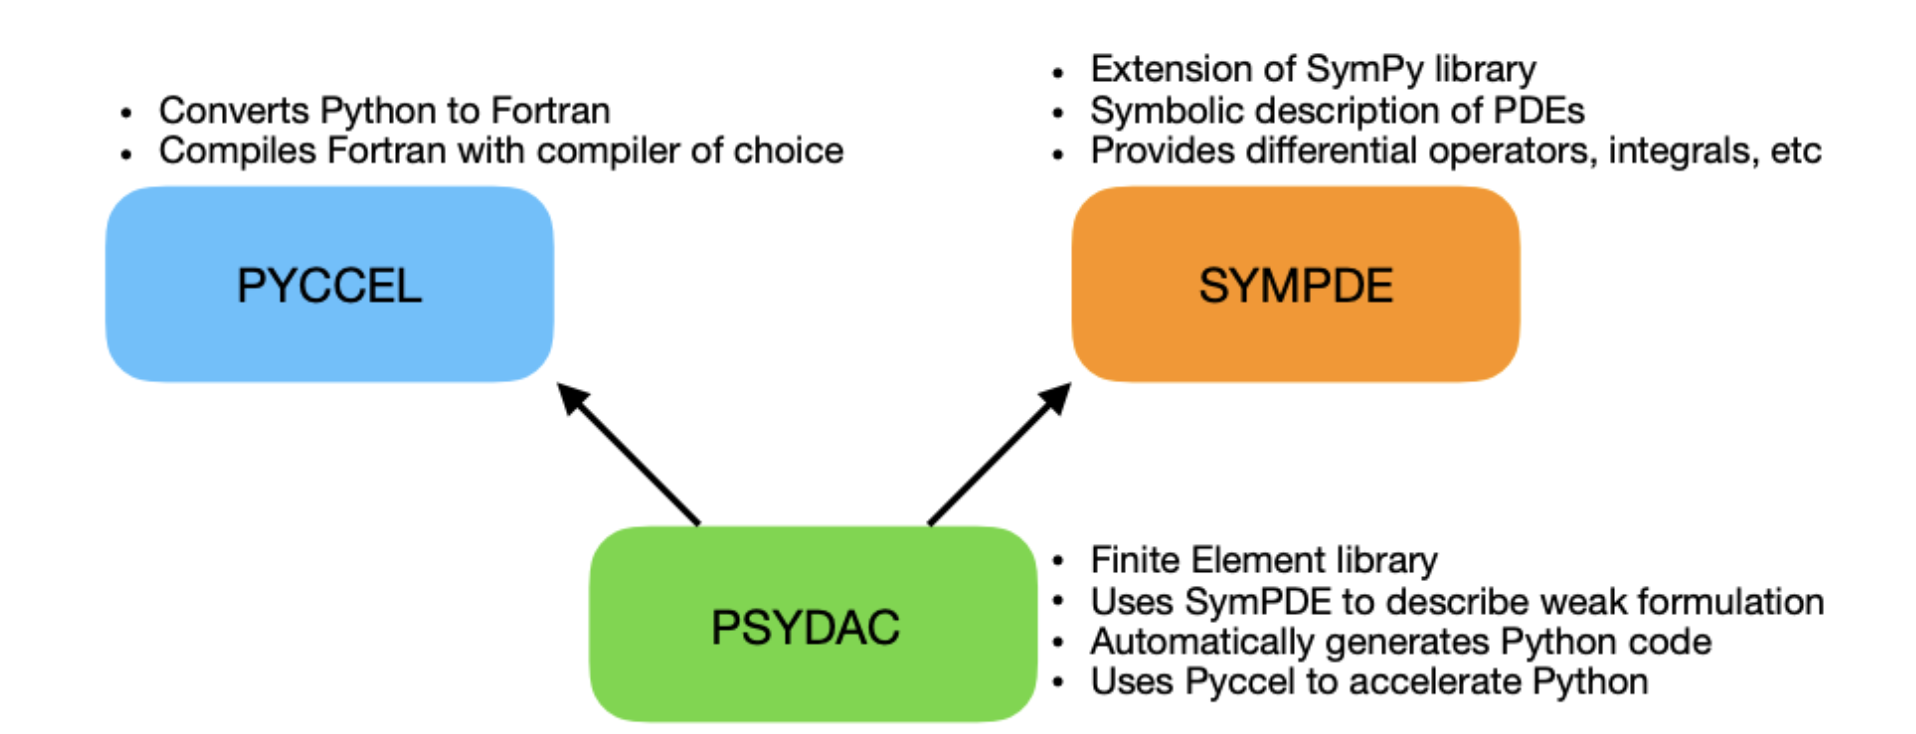
\includegraphics[width=0.75\linewidth]{psydac_fonc_1.png}
    \caption{Dependancy graph of \texttt{PSYDAC}, from \cite{guclu_psydac_2022}}
    \label{fig:Dependancy_Psydac}
\end{figure}

Raven is a supercomputer located at the Max-Planck Institute for Plasma Physics. It is part of the High Performance Computing (HPC) infrastructure and is used for large-scale simulations and data analysis in plasma physics and related fields. I had the opportunity to run my simulations on Raven, which provided me with access to powerful computational resources and parallel processing capabilities.

\subsection{Dirichlet Homogeneous Boundary conditions on $\partial\Omega_D = \partial\Omega$} \label{subsec:Dirichlet Homogeneous Boundary conditions on}

In a first time, to get the grips with \texttt{PSYDAC} and the HPC, I have considered the case $\Omega = [0,1]^3$, $\partial \Omega_D = \partial\Omega$ and $\partial \Omega_N = \emptyset$. To verify if the numerical resolution of \texttt{PSYDAC} of \eqref{eq:weakdisplacementform} is correct, I have used the Method of Manufactured Solutions. The concept is quite simpler, we assume that a function $\vec u_e \in \boldsymbol H^1_{\vec 0}(\Omega)$ verifies the strong problem \eqref{eq:strong_form}, then we compute the source term $\vec f$ and we solve the \eqref{eq:weakdisplacementform} with $\vec f$ as a source term and we look at the error between the numerical solution and the theoretical one.
I have considered $\vec u_e$ defined as : $$\vec u_e = \begin{pmatrix}
    0 \\
    0 \\
\sin{\left(\pi x \right)} \sin{\left(\pi y \right)} \sin{\left(\pi z \right)}
\end{pmatrix} \in \boldsymbol H^1_{\vec 0}(\Omega).$$ Then, we can compute manually the source term $\vec f$ : $$\vec f = \begin{pmatrix}
     - \pi^{2} \left(\lambda + \mu\right) \sin{\left( y \right)} \cos{\left(\pi x \right)} \cos{\left(\pi z \right)} \\
     - \pi^{2} \left(\lambda + \mu\right) \sin{\left(\pi x \right)} \cos{\left( y \right)} \cos{\left(\pi z \right)} \\  
      \pi^{2} \left(\lambda + 4 \mu\right) \sin{\left(\pi x \right)} \sin{\left(\pi y \right)} \sin{\left(\pi z \right)}
\end{pmatrix} \in \boldsymbol L^2(\Omega).$$

To make the numerical simulation with \texttt{PSYDAC}, we have to choose two important parameters : $d$ the maximum degree of B-Splines functions that will approximate the solution and $n_{\text{cells}}$ is the number of cells in each dimension of $\Omega$ for the finite dimensional space. $\displaystyle h \propto \frac{1}{n_{\text{cells}}}$, an usual discretization parameters for finite dimensional spaces and $d$ will conduct the convergence speed of the numerical solution. 
By solving the problem Dirichlet Homogeneous Boundary conditions on the whole border, one can observe the following plots of the simulated $\vec u_{e,3}^h$ for different plane $z$. It is possible to plot also the error $\vec u_{e,3} - \vec u_{e,3}^h$.

\newpage

\begin{figure}
    \centering
    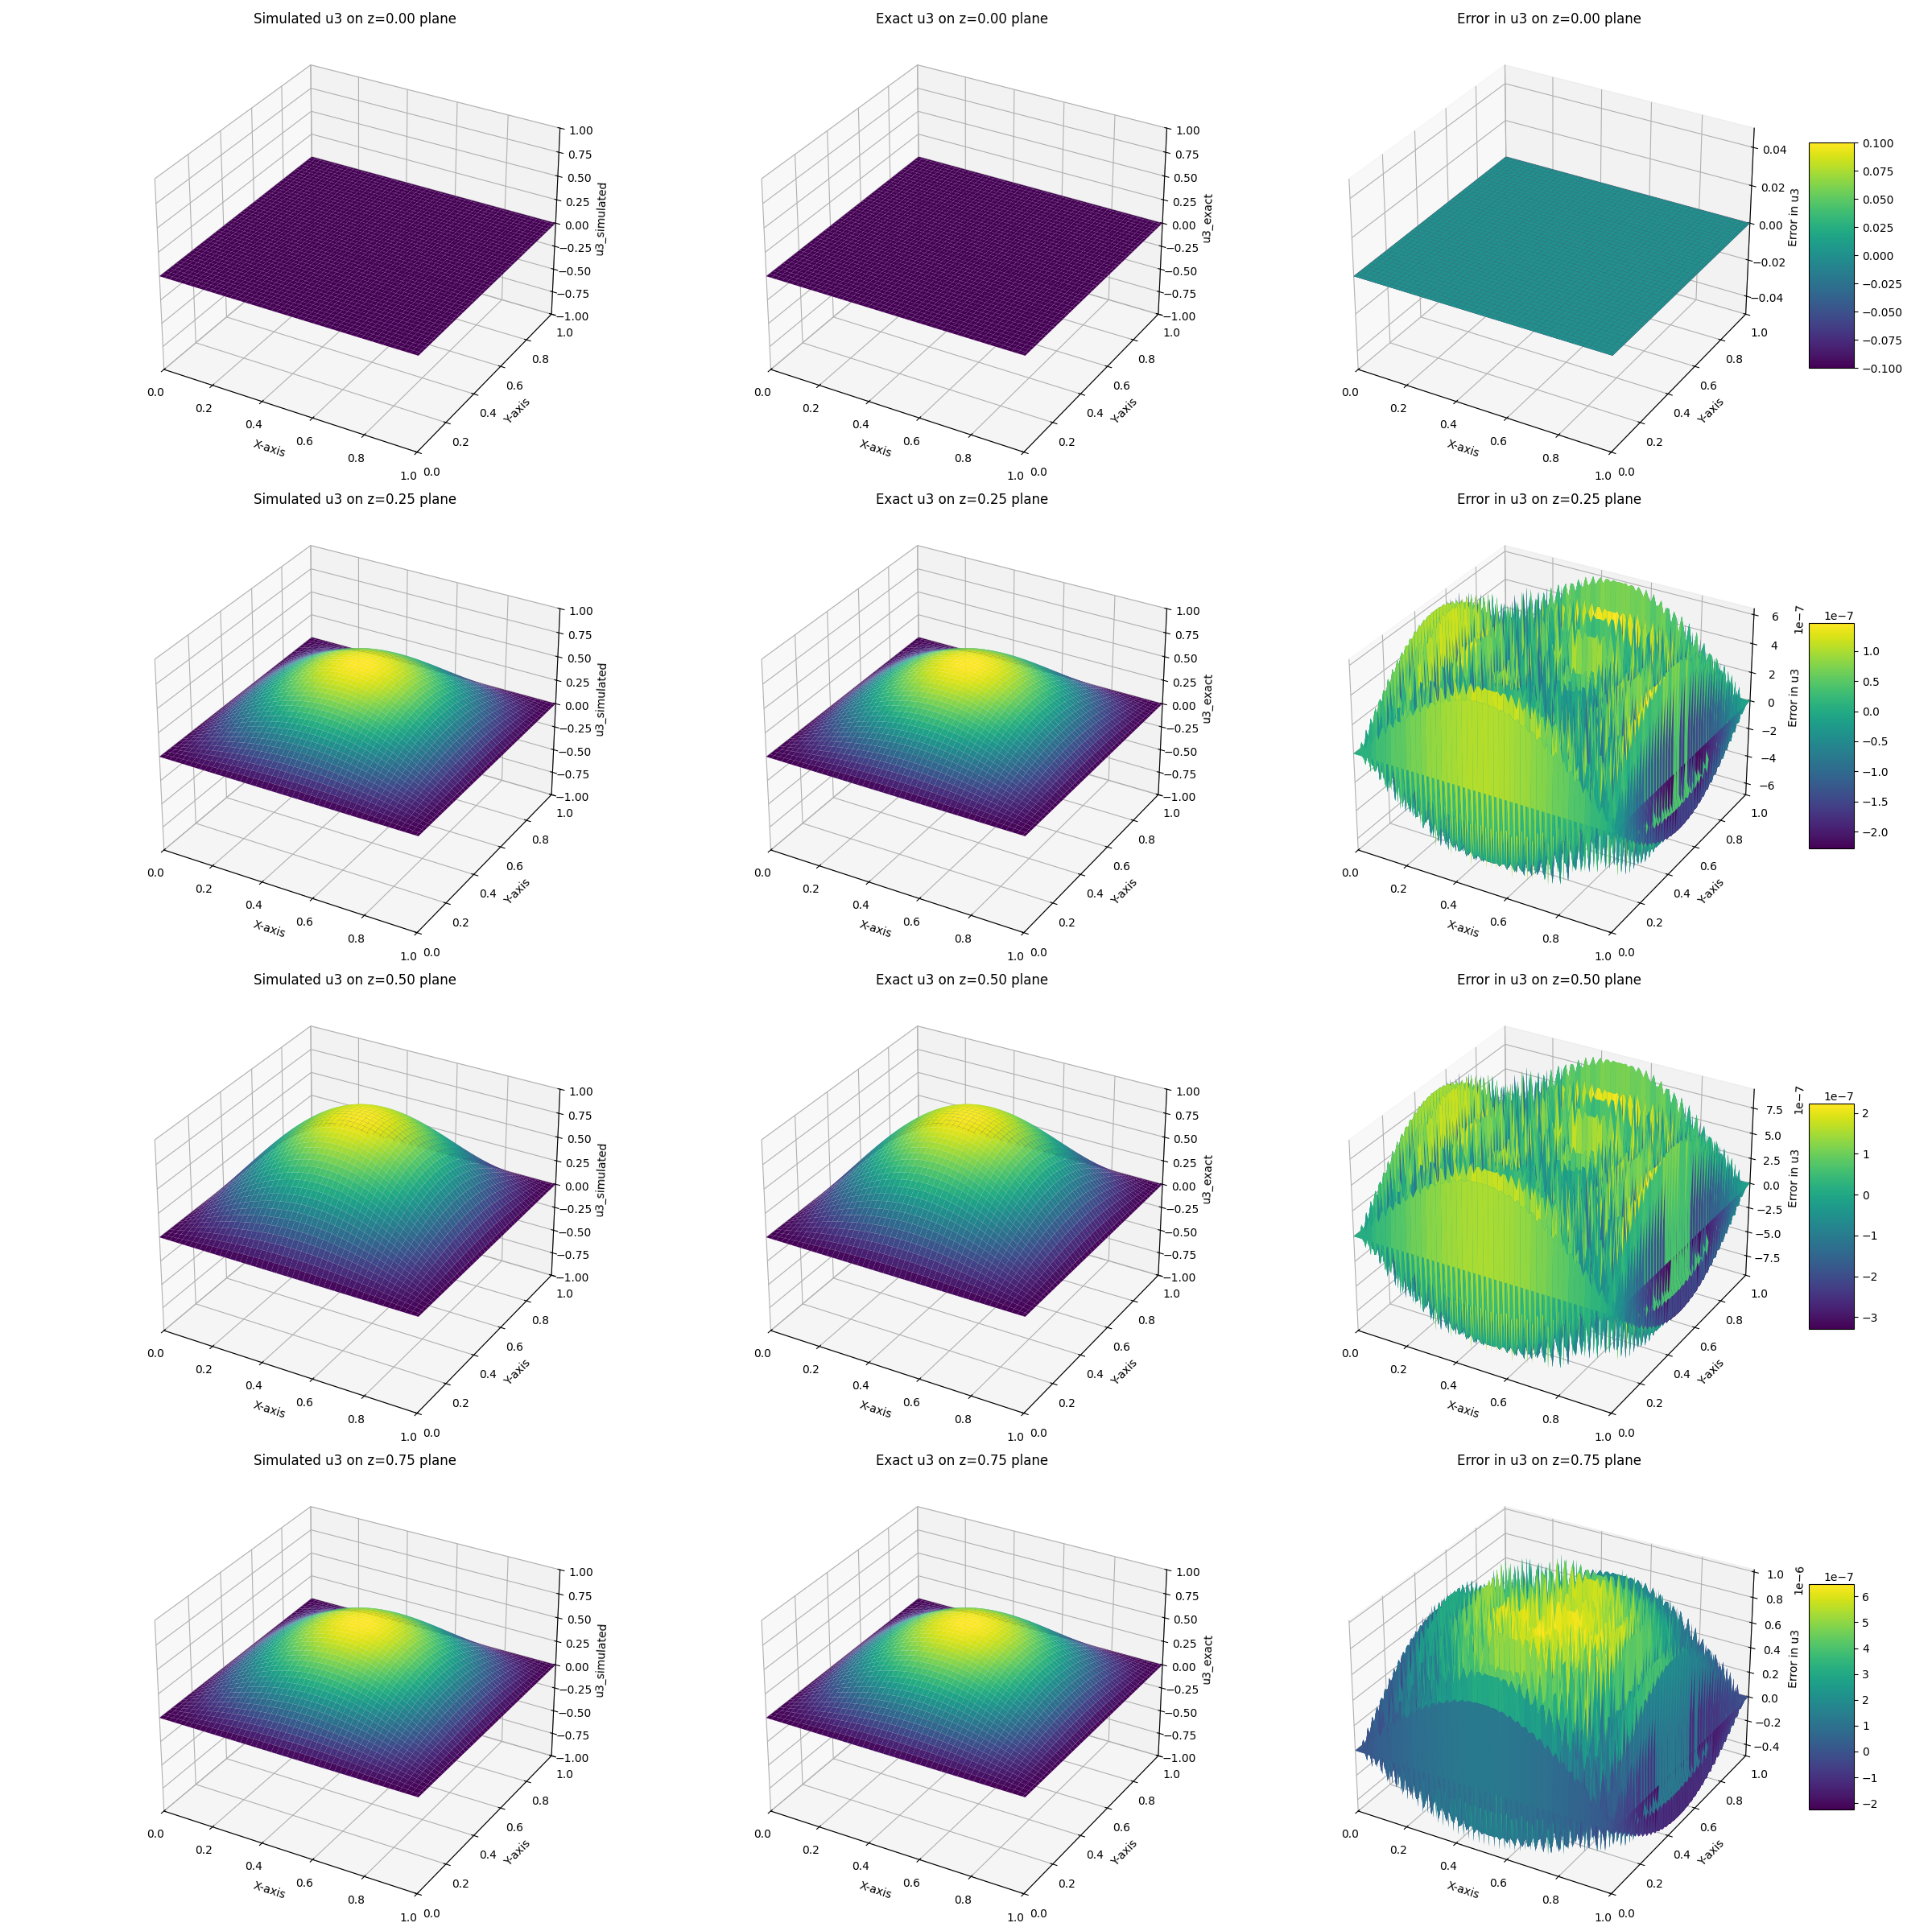
\includegraphics[width=0.9\linewidth]{3d_plots_degree_2_non_mixed_dirichlet_homogeneous_ncell=64.png}
    \caption{Plots comparison between the simulated and real $u_{e,3}$ with the error, for different plane $z$, with $d=2$ and $n_{\text{cell}} = 64$}
    \label{fig:3D_plots}
\end{figure}

We can observe that the numerical solution is "quite" near the real solution. To get a better estimation of convergence rate, let's look at the Céa's lemma in this case.

Denotes by $\boldsymbol V^h \subset \boldsymbol H^1(\Omega)$ the discrete finite dimensional space, $\vec u \in \boldsymbol H^{s+1}(\Omega) \subset \boldsymbol H^1(\Omega), 1 \leq s \leq d+1$ the real solution solution and $\vec u^h \in \boldsymbol V^h$ the discrete solution.
Then, the Céa's lemma gives the following estimates : 
$$\norm{\vec u - \vec u^h}_{\boldsymbol H^1(\Omega)} \leq \frac{3\lambda + 2\mu}{2\mu C} \inf_{\vec v^h \in \boldsymbol H^1(\Omega)} \norm{\vec u - \vec v^h}_{\boldsymbol H^1(\Omega)}$$
\textit{where $C > 0$ is a constant from Korn's inequality (independant of $h$).}
By applying \textbf{Corollary 4.21, 4.27}, \textbf{Theorem 6.2} from \cite{da_veiga_mathematical_2014} and Aubin-Nitsche theorem, we can get the following estimates : 
\begin{equation}
\begin{aligned}
& \norm{\vec u - \vec u^h}_{\boldsymbol H^1(\Omega)} \lesssim \frac{3\lambda + 2\mu}{2\mu C} h^q \norm{\vec u}_{\boldsymbol H^{q+1}(\Omega)} \\
& \norm{\vec u - \vec u^h}_{\boldsymbol L^2(\Omega)} \lesssim (3\lambda + 2\mu) h^{q+1}\norm{\vec u}_{\boldsymbol H^{q+1}(\Omega)}
\end{aligned}
\label{eq:convergence_estimates}
\end{equation}
\textit{where $q = \min{(s,d)}$}. In this case, $u_e$ is an infinitly smooth solution, then $q = d$. 

\begin{figure}[!h]
	\centering
	\begin{subfigure}[b]{0.49\textwidth}
		\centering
		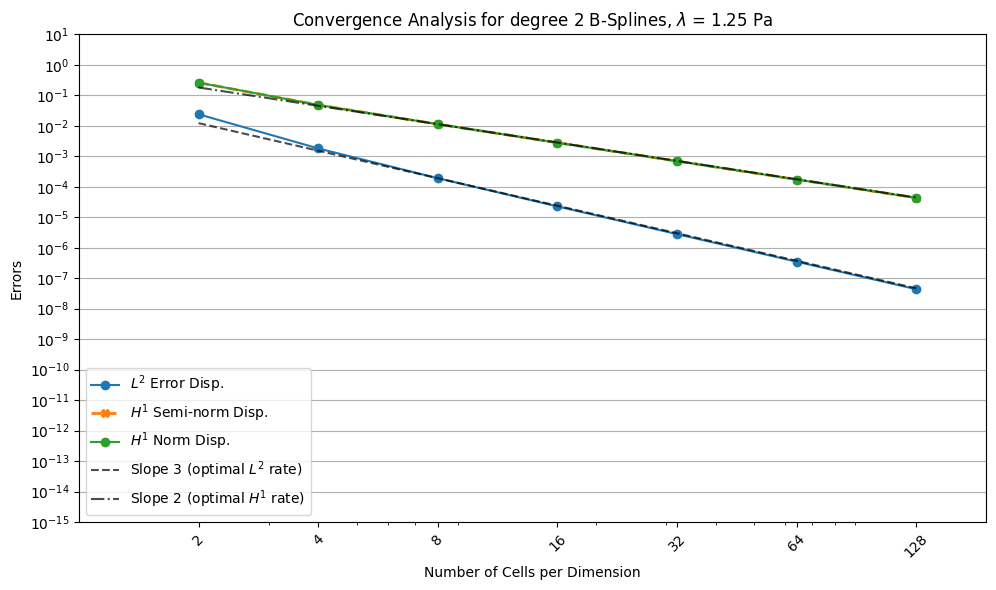
\includegraphics[width=\textwidth]{figures_non_mixed_DH/convergence_plot_degree_2_lambda=1.25.png}
		\caption{$d=2$}
		\label{fig:deg2_NMDHBC}
	\end{subfigure}
	\begin{subfigure}[b]{0.49\textwidth}
		\centering
		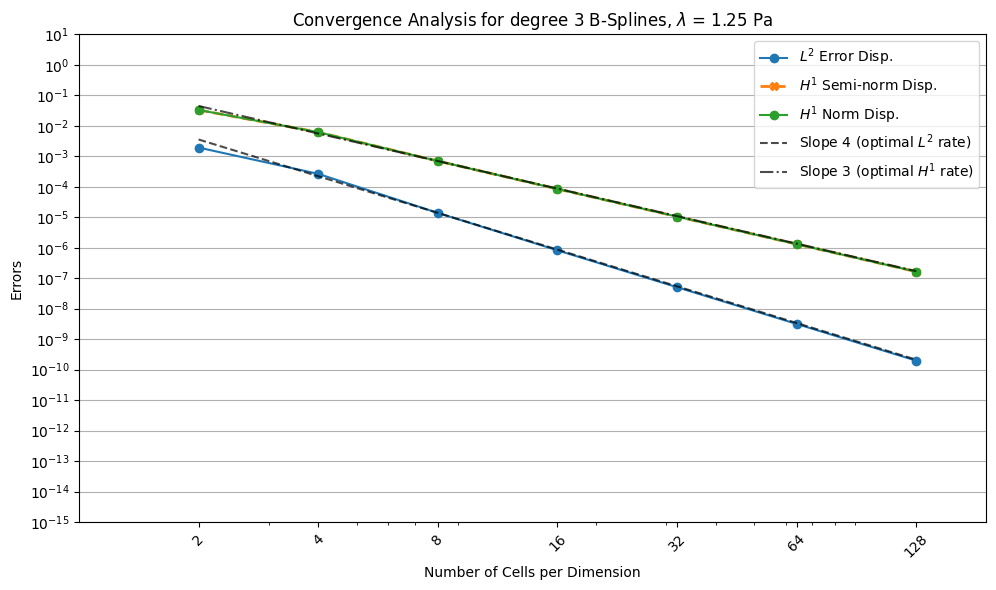
\includegraphics[width=\textwidth]{figures_non_mixed_DH/convergence_plot_degree_3_lambda=1.25.png}
		\caption{$d=3$}
		\label{fig:deg3_NMDHBC}
	\end{subfigure}
	\\
	\begin{subfigure}[b]{0.49\textwidth}
		\centering
		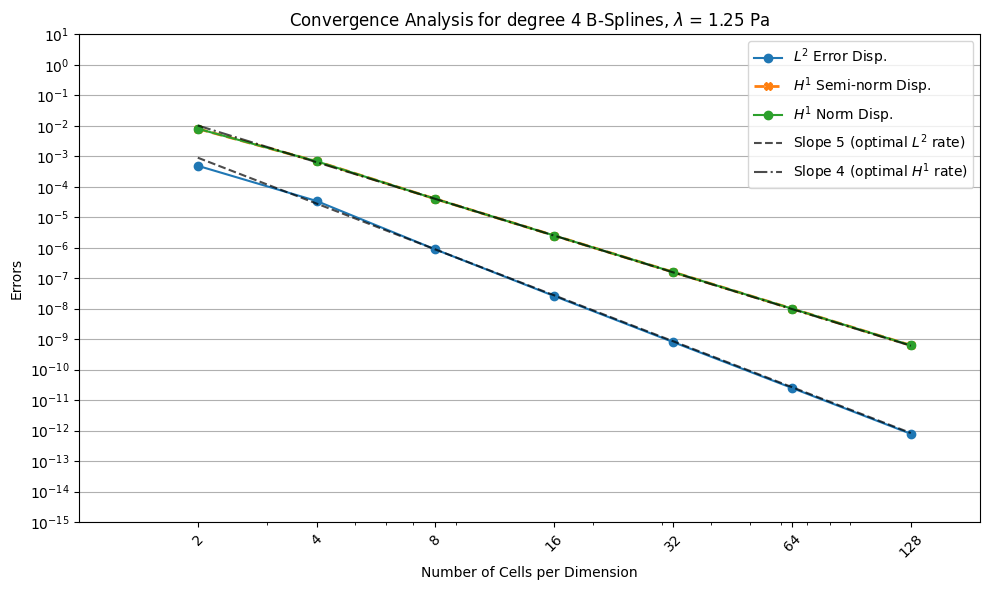
\includegraphics[width=\textwidth]{figures_non_mixed_DH/convergence_plot_degree_4_lambda=1.25.png}
		\caption{$d=4$}
		\label{fig:deg4_NMDHBC}
	\end{subfigure}
	\begin{subfigure}[b]{0.49\textwidth}
		\centering
		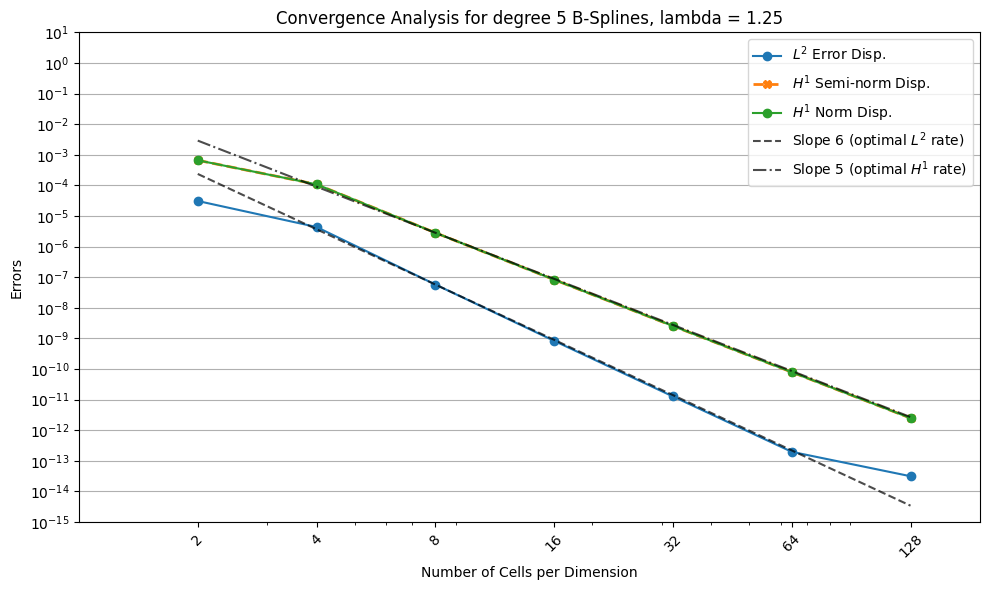
\includegraphics[width=\textwidth]{figures_non_mixed_DH/convergence_plot_degree_5_lambda=1.25.png}
		\caption{$d=5$}
		\label{fig:deg5_NMDHBC}
	\end{subfigure}
	\caption{Four plots of relative errors ($\norm{\vec u - \vec u^h}_{\boldsymbol H^1(\Omega)}$ and $\norm{\vec u - \vec u^h}_{\boldsymbol L^2(\Omega)}$) with different degree B-Splines (with $\lambda = 1.25$  \& $\mu = 1$)}
	\label{fig:four_errors_graphs}
\end{figure}

We can see that the numerical solution converges with the expected order to the real solution : the more the mesh is refined, the more the error is lower and the more the splines' degree is higher, the more the convergence rate is higher. 
For this numerical resolution, I have used \textbf{GMRES} method to solve the linear system at the end of the discretization. That needed to take care of the tolerance of the solver, because with a fixed tolerance, if the $d$ and $n_{\text{cells}}$ are "too higher", the convergence rate cannot hold. The following figure illustrates this case, when $d=5$ and $n_{\text{cells}} = 16$.

\begin{figure}[!h]
	\centering
	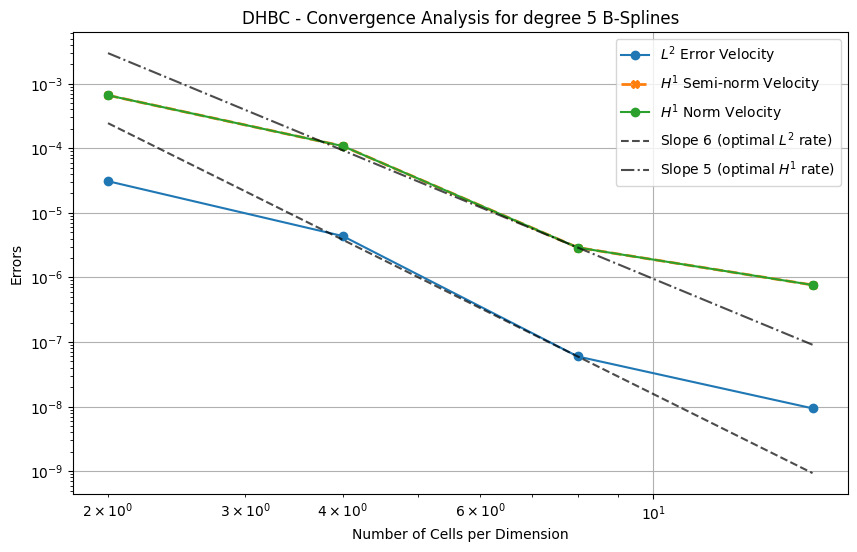
\includegraphics[width=0.5\linewidth]{degre5_nul}
	\caption{Error plot between exact and numerical solution with degree 5 B-Splines with "higher" tolerance for the solvera}
\end{figure}

But even with a lower tolerance for the solver ($10^{-15}$ for figure \ref{fig:deg5_NMDHBC}), the error reaches a plateau, which is not the case for lower degree B-Splines (at least for the tested configurations).

\subsection{Mixed boundary conditions}

Then, I have made a simulation with Mixed Boundary Conditions, as it is introduced in \eqref{eq:strong_form}, with also non-homogeneous dirichlet boundary conditions.

Again, $\Omega = [0,1]^3$, with : 
\begin{equation*}
	\begin{aligned}
		& \partial \Omega_{\text{DH}} = \left\{  (x,y,z) \in \partial\Omega \left| z = 0 \text{ or } z = 1 \right.  \right\} \\ 
		& \partial \Omega_{\text{DNH}} = \left\{  (x,y,z) \in \partial\Omega \left| x = 0 \text{ or } x = 1 \right.  \right\} \\
		& \partial \Omega_{\text{N}} = \left\{  (x,y,z) \in \partial\Omega \left| y = 0 \text{ or } y = 1 \right.  \right\}.
	\end{aligned}
\end{equation*}
For that purpose, $\vec u_e, \vec f, \vec t_N$ and $\vec g$ are now defined as : 
\begin{equation*}
\begin{aligned}
	& \vec u_e =
	\begin{pmatrix}
		0 \\  
		0 \\ 
		\sin{\left(\pi z \right)} \cos{\left(\pi x \right)} \cos{\left(\pi y \right)}
	\end{pmatrix}, \hfill \vec f =  \begin{pmatrix}
	\pi^{2} \left(\lambda + \mu\right) \sin{\left(\pi x \right)} \cos{\left(\pi y \right)} \cos{\left(\pi z \right)} \\
	\pi^{2} \left(\lambda + \mu\right) \sin{\left(\pi y \right)} \cos{\left(\pi x \right)} \cos{\left(\pi z \right)} \\
	\pi^{2} \left(\lambda + 4 \mu\right) \sin{\left(\pi z \right)} \cos{\left(\pi x \right)} \cos{\left(\pi y \right)}
	\end{pmatrix} \\
	& \vec t_N = \begin{pmatrix}
	0 \\  
	- \lambda \pi \cos{\left(\pi x \right)} \cos{\left(\pi z \right)} \\  
	0
	\end{pmatrix}, \hfill \vec g = \begin{pmatrix}
	0 \\  
	0 \\ 
	\pm \sin{\left(\pi z \right)} \cos{\left(\pi y \right)}
	\end{pmatrix}
\end{aligned}
\end{equation*}	

Then, we can get the same plots and interpretation as before. 

\begin{figure}[!h]
	\centering
	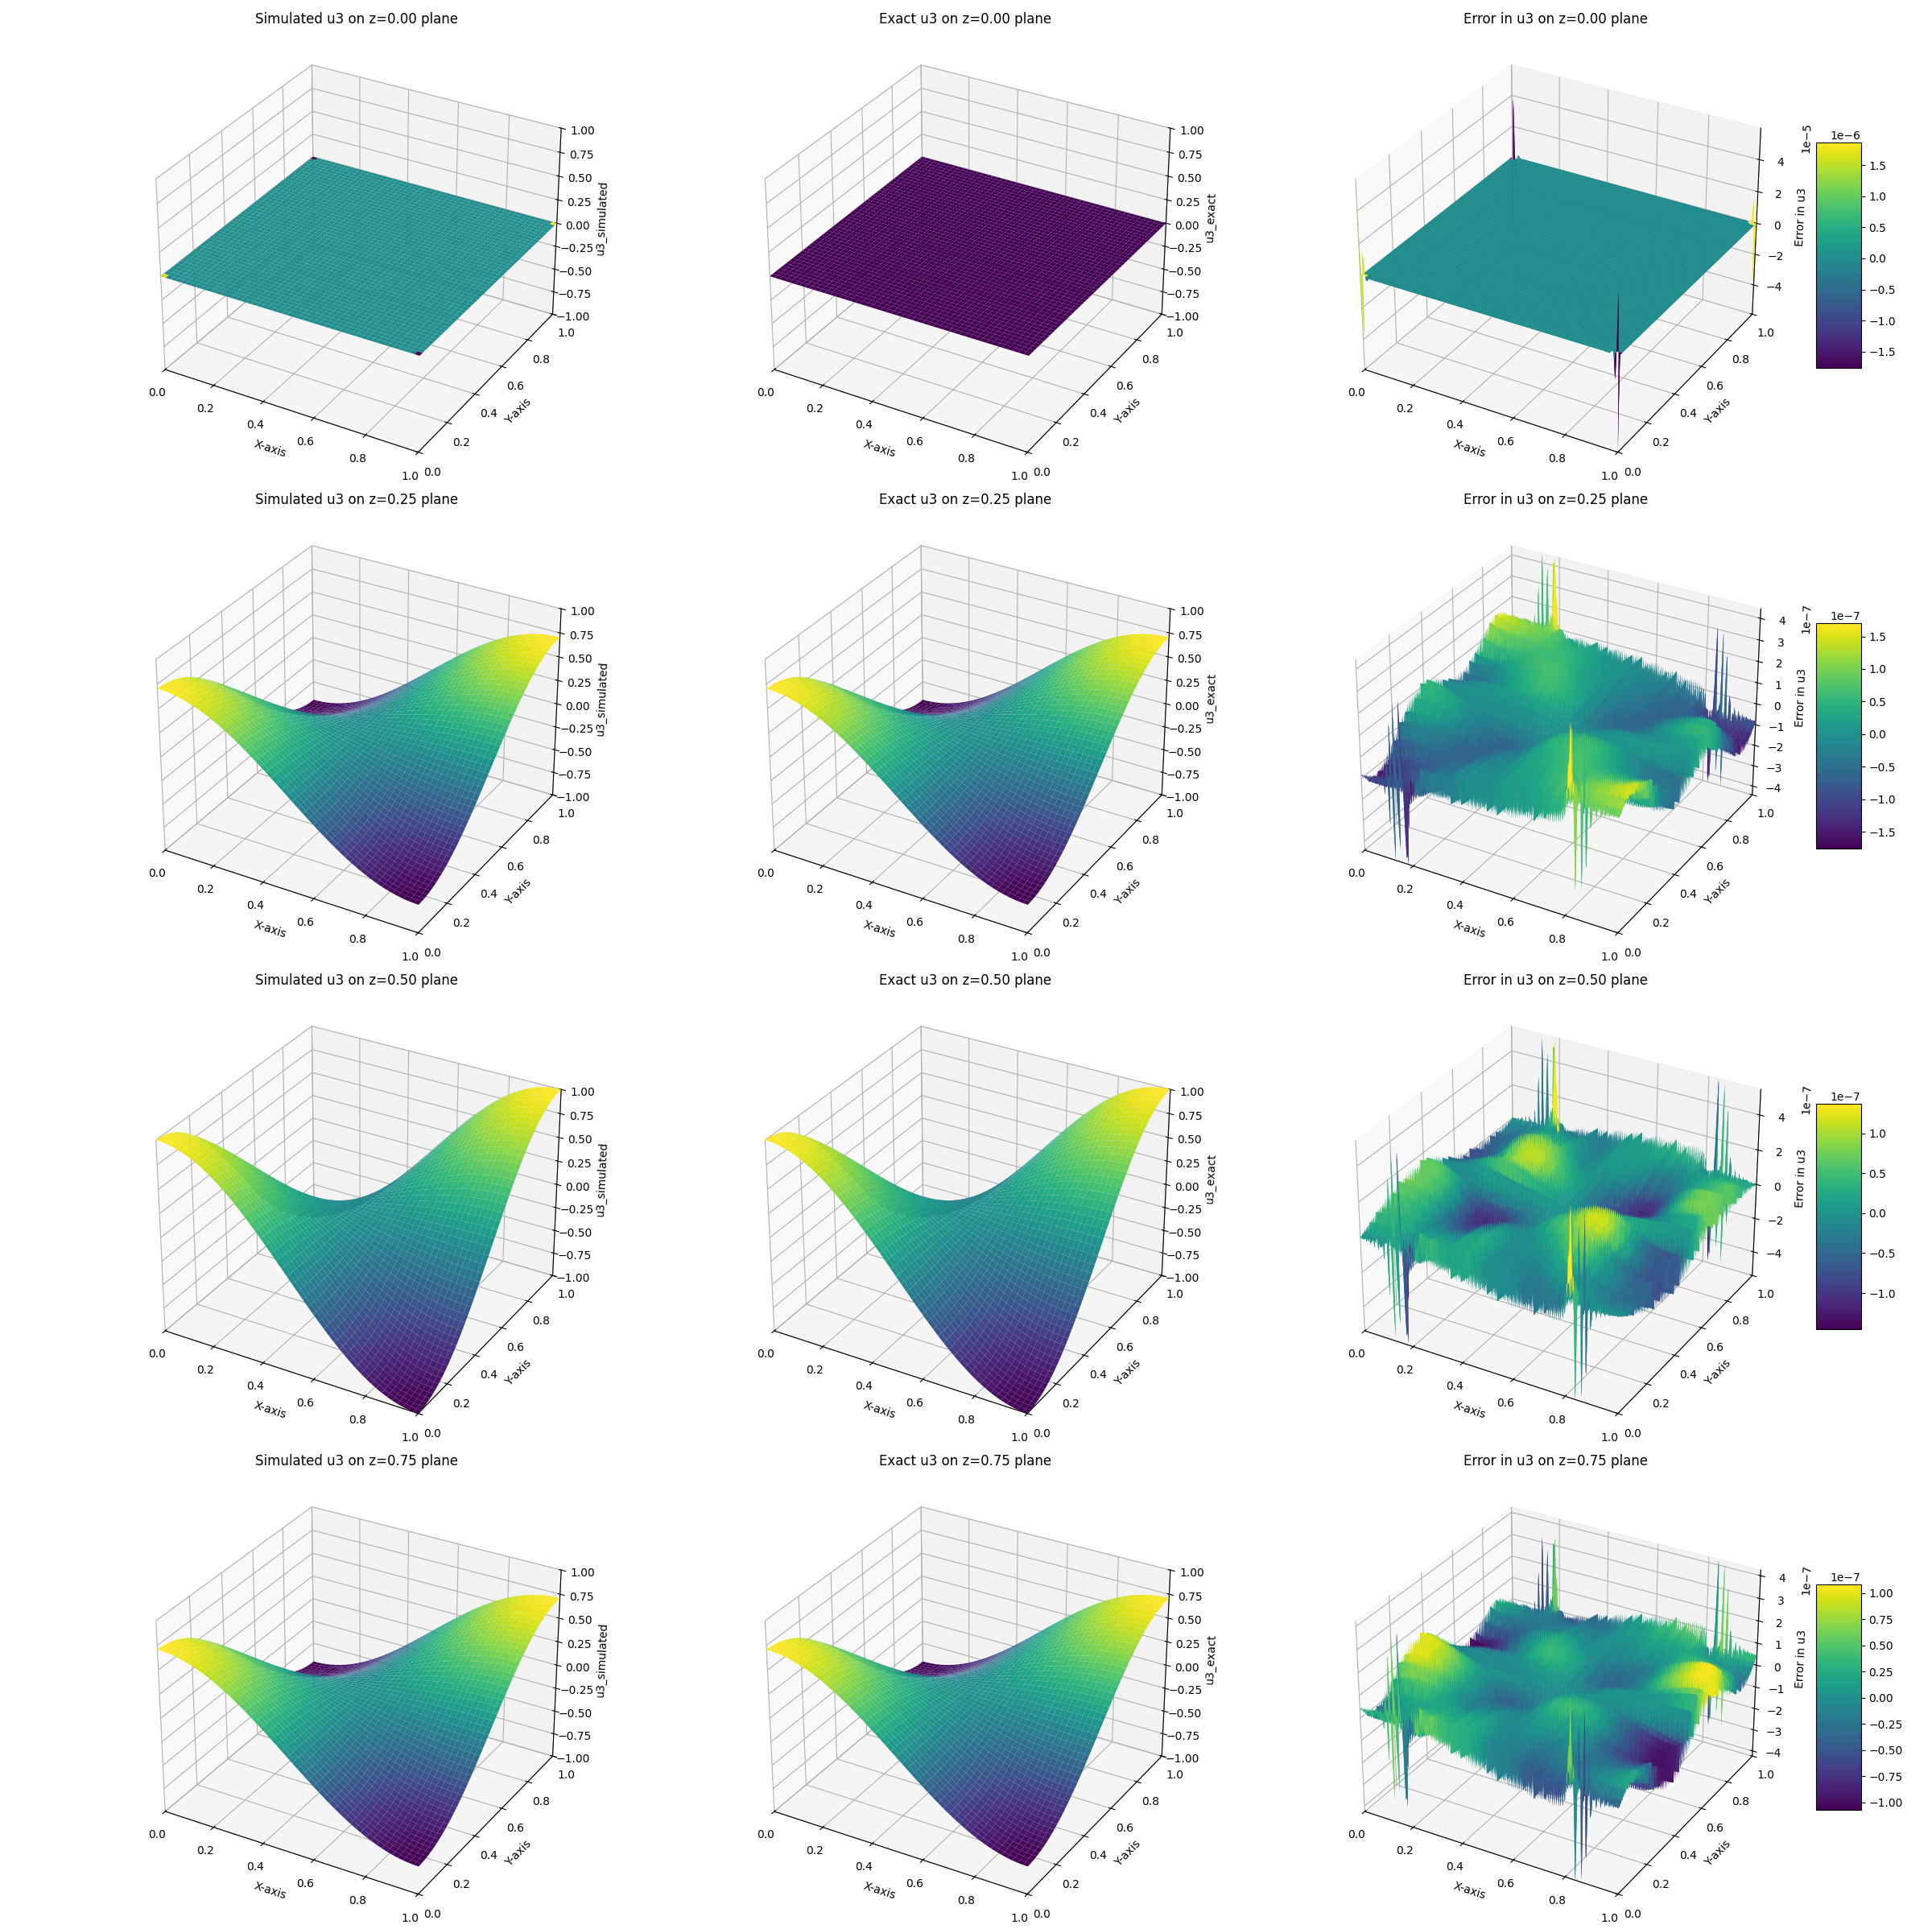
\includegraphics[width=0.7\linewidth]{3d_plots_degree_2_non_mixed_ncell=128_function_u3_planes_z.png}
	\caption{Plots comparison between the simulated and real $u_{e,3}$ with the error, for different plane $z$, with $d=2$ and $n_{\text{cell}} = 128$}
	\label{fig:3D_plots_mixed_BC}
\end{figure}

\begin{figure}[!h]
	\centering
	\begin{subfigure}[b]{0.49\textwidth}
		\centering
		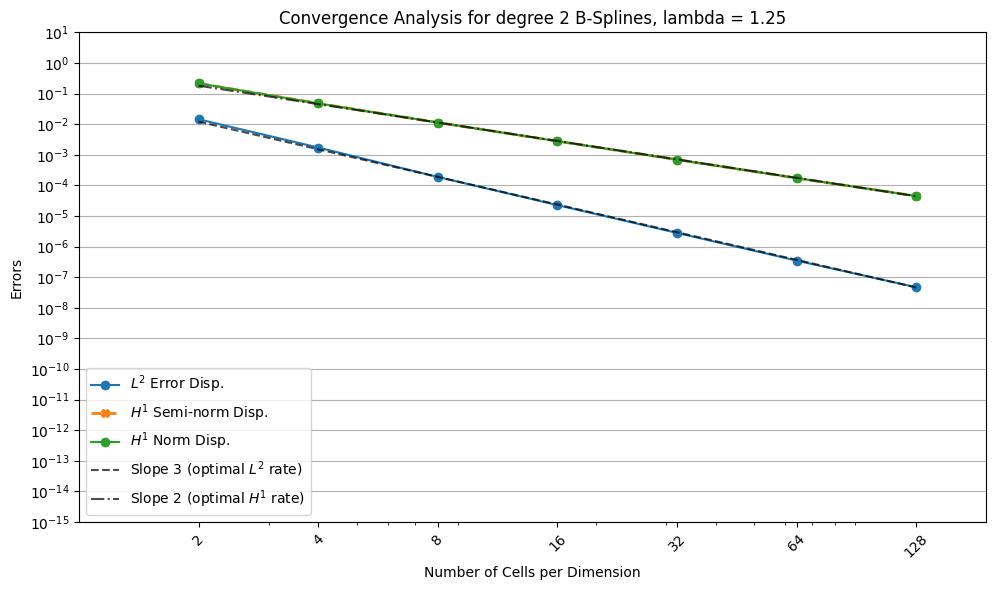
\includegraphics[width=\textwidth]{figures_non_mixed/convergence_plot_degree_2_lambda=1.25.png}
		\caption{$d=2$}
		\label{fig:deg2_NM}
	\end{subfigure}
	\begin{subfigure}[b]{0.49\textwidth}
		\centering
		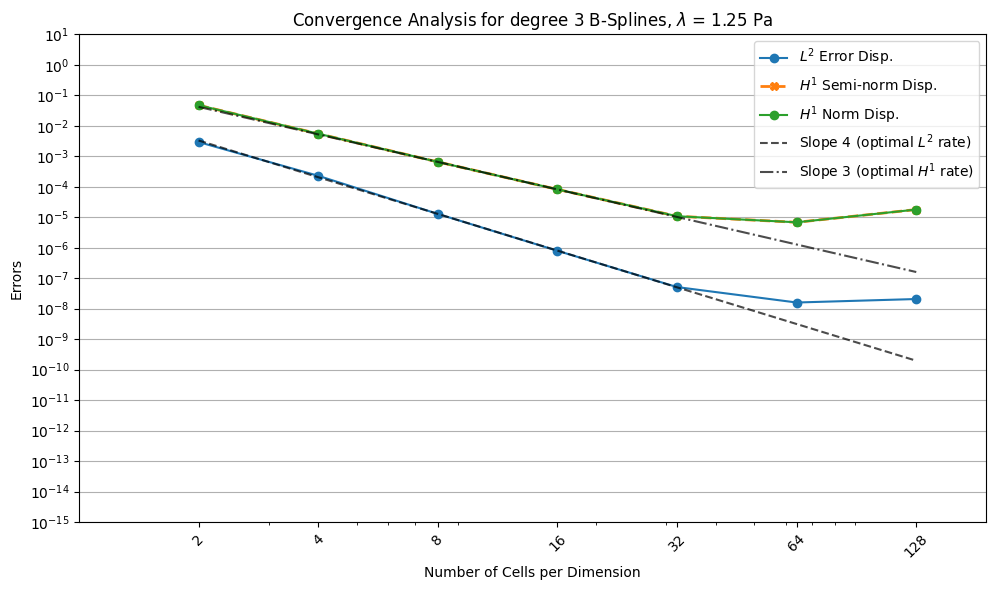
\includegraphics[width=\textwidth]{figures_non_mixed/convergence_plot_degree_3_lambda=1.25.png}
		\caption{$d=3$}
		\label{fig:deg3_NM}
	\end{subfigure}
	\\
	\begin{subfigure}[b]{0.49\textwidth}
		\centering
		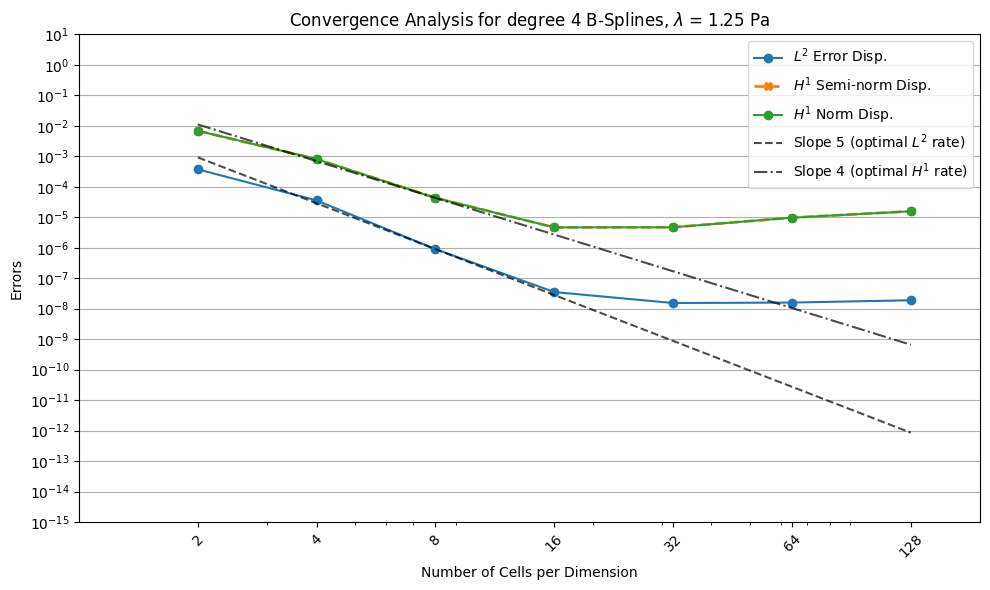
\includegraphics[width=\textwidth]{figures_non_mixed/convergence_plot_degree_4_lambda=1.25.png}
		\caption{$d=4$}
		\label{fig:deg4_NM}
	\end{subfigure}
	\begin{subfigure}[b]{0.49\textwidth}
		\centering
		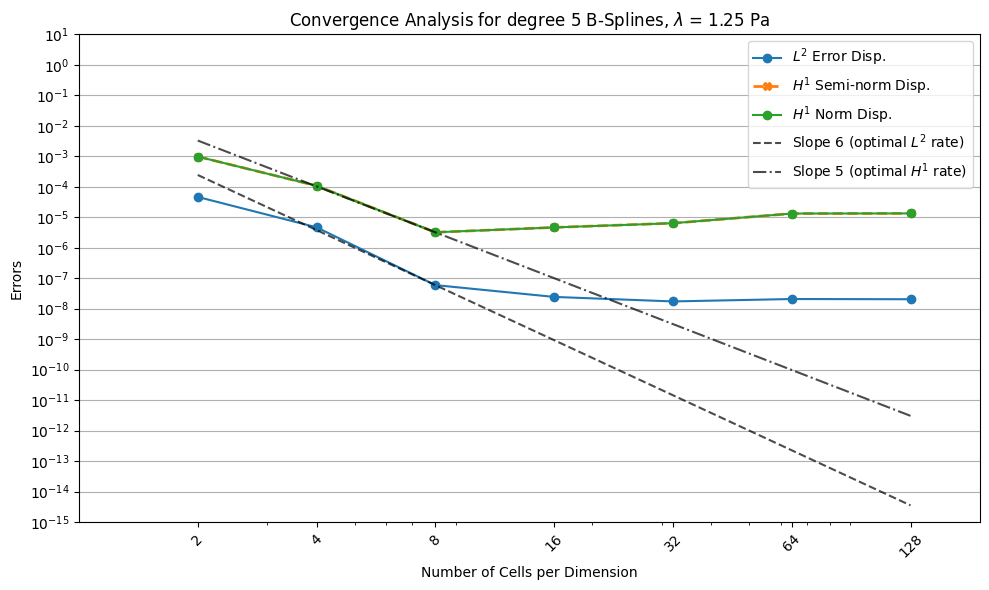
\includegraphics[width=\textwidth]{figures_non_mixed/convergence_plot_degree_5_lambda=1.25.png}
		\caption{$d=5$}
		\label{fig:deg5_NM}
	\end{subfigure}
	\caption{Four plots of relative errors ($\norm{\vec u - \vec u^h}_{\boldsymbol H^1(\Omega)}$ and $\norm{\vec u - \vec u^h}_{\boldsymbol L^2(\Omega)}$) with different degree B-Splines (with $\lambda = 1.25$  \& $\mu = 1$)}
	\label{fig:four_errors_graphs}
\end{figure}

\newpage 
For fixed value $\lambda = 1.25$ and $\mu = 1$, the codes seems to give a numerical solution that converges to the theoritical one with the expected order. 

But, the estimates \eqref{eq:convergence_estimates} depends on $\frac{\lambda}{\mu}$, and when $\lambda \rightarrow + \infty$ (which is the case for incompressible material), the estimates doesn't hold. Numerically, it is hard to get a value goes to $+\infty$, but for increasing values of $\lambda$, we can get plots from figure \ref{fig:error_kappa} below. 

\begin{figure}[!h]
	\centering
	\begin{subfigure}[b]{0.49\textwidth}
		\centering
		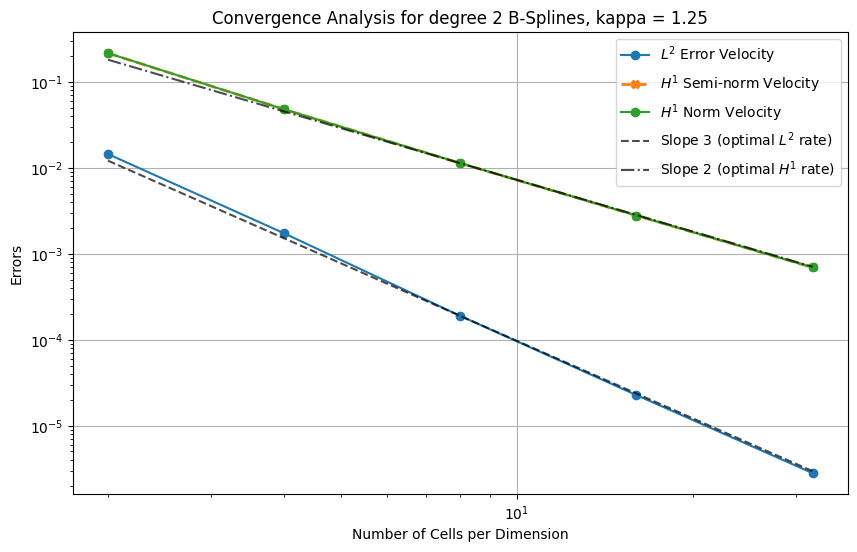
\includegraphics[width=\textwidth]{convergence_degree_2_non_mixed_kappa=1.25}
		\caption{$\lambda=1.25$}
	\end{subfigure}
	\begin{subfigure}[b]{0.49\textwidth}
		\centering
		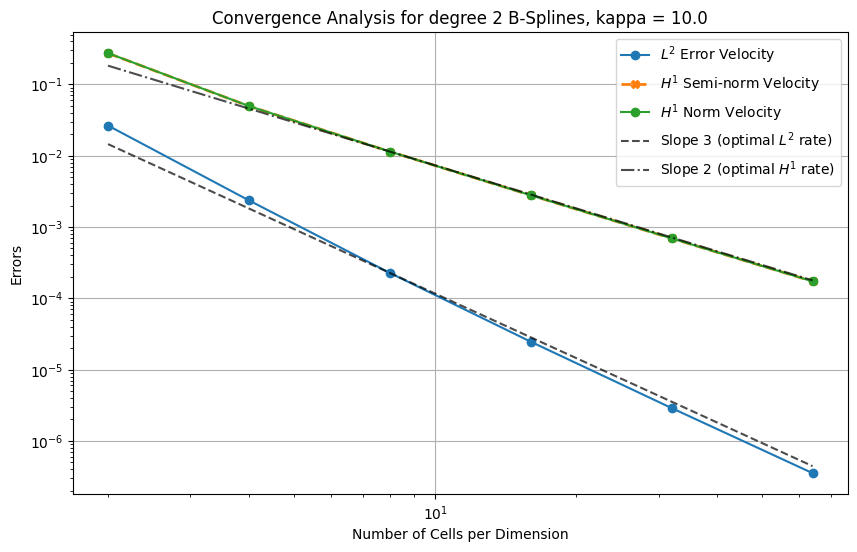
\includegraphics[width=\textwidth]{convergence_degree_2_non_mixed_kappa=10.0}
		\caption{$\lambda=10$}
	\end{subfigure}
\end{figure}
\begin{figure}[!h]
	\centering
	\begin{subfigure}[b]{0.49\textwidth}
		\centering
		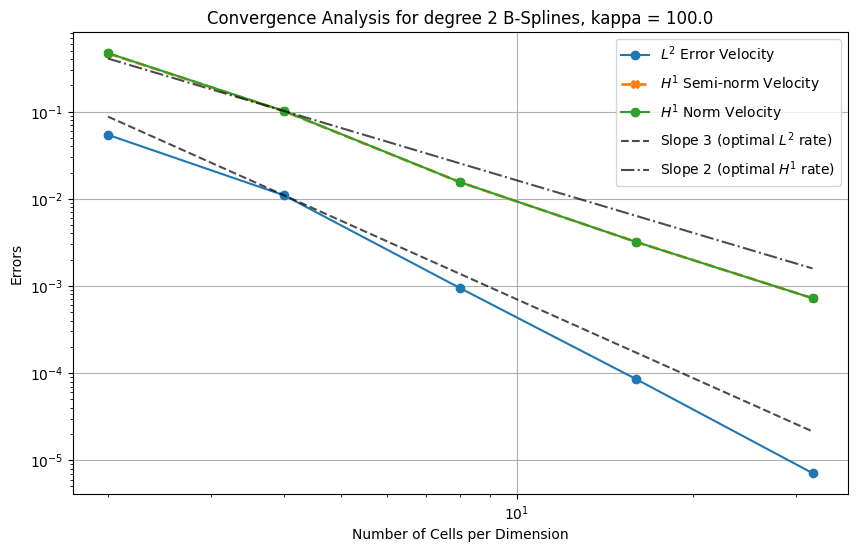
\includegraphics[width=\textwidth]{convergence_degree_2_non_mixed_kappa=100.0}
		\caption{$\lambda=100$}
	\end{subfigure}
	\begin{subfigure}[b]{0.49\textwidth}
		\centering
		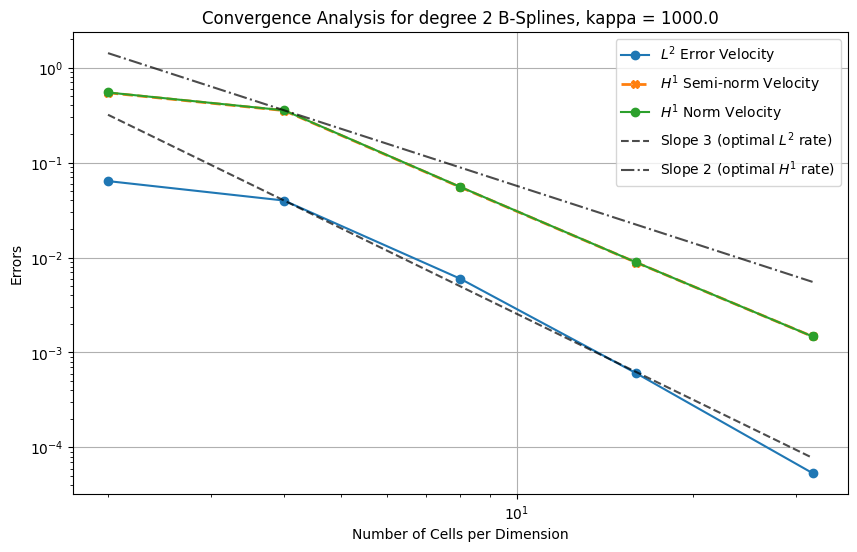
\includegraphics[width=\textwidth]{convergence_degree_2_non_mixed_kappa=1000.0}
		\caption{$\lambda=1000$}
	\end{subfigure}
	\\
	\begin{subfigure}[b]{0.49\textwidth}
		\centering
		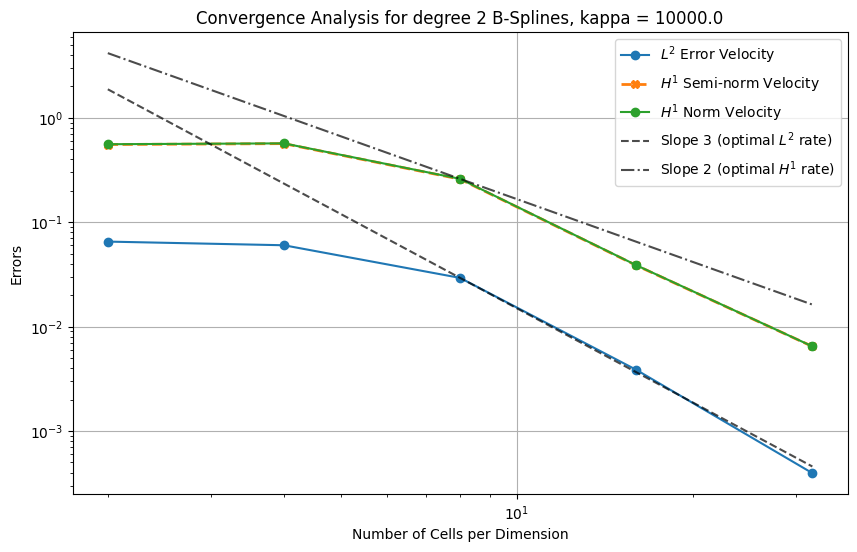
\includegraphics[width=\textwidth]{convergence_degree_2_non_mixed_kappa=10000.0}
		\caption{$\lambda=10000$}
	\end{subfigure}
	\begin{subfigure}[b]{0.49\textwidth}
		\centering
		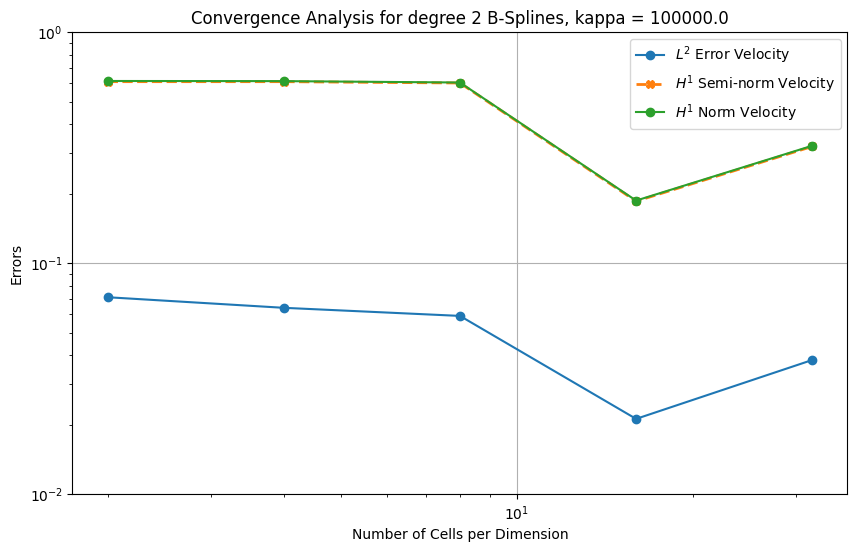
\includegraphics[width=\textwidth]{convergence_degree_2_non_mixed_kappa=100000.0}
		\caption{$\lambda=100000$}
	\end{subfigure}
	\caption{Error plots between exact solution and numerical solution with degree 2 B-Splines with increasing values of $\lambda$ with $\mu = 1$}
	\label{fig:error_kappa}
\end{figure}


\newpage

To compensate the problem of high values of $\lambda$, I have proposed to explore a Mixed Formulation by introducing a pressure field.


\section{Mixed displacement-pressure formulation}
To introduce this formulation, let's consider again the strong formulation from \eqref{eq:strong_form}. Then, denotes by $p$ the pressure field, defined by $\displaystyle p = - \lambda \div{\vec u}$. As we are seeking $\vec u \in \boldsymbol{H}^1(\Omega)$, $p$ is naturally living in $L^2(\Omega)$. Then Hook's law can be rewritten : $\boldsymbol{\sigma} (\vec u,p) = -p I_3 + 2\mu \boldsymbol{\varepsilon(\vec u} \text{ in }  \Omega $ \\
So the strong formulation can be re-write as : For a given $\vec f \in \boldsymbol L^2(\Omega)$, $\vec t_N \in \boldsymbol L^2(\partial \Omega_N)$, find $(\vec u, p) \in \boldsymbol H^1(\Omega)\times L^2(\Omega)$ such that : 

\begin{equation}
	\label{eq:strong_pressure_disp_form}
	\left \{
	\begin{aligned}
		& - \div \boldsymbol{\sigma} (\vec u,p) = \vec f & \text{ in } & \Omega \hspace{1cm} \text{(Equilibrium)}\\
		& \div{\vec u} + \frac{1}{\lambda} p = 0 & \text{ in } & \Omega \hspace{1cm} \text{(Pressure field definition)} \\
		& \vec u = \vec 0 & \text{ in } &\partial \Omega_D \\
		& \boldsymbol{\sigma} (\vec u) \cdot \vec n = \vec t_N & \text{ in }& \partial \Omega_N
	\end{aligned}
	\right.
\end{equation}

Now, to derive the weak formulation associated, first we multiply the Equilibrium equation by $v \in \boldsymbol H^1_{\vec 0,D}(\Omega)$ and we interger by part on $\Omega$, then we multiply the Pressure field equation by $q \in L^2(\Omega)$ and we interger over $\Omega$. Then we just have to add both integrals. 
Then, the weak formulation is: 
\begin{equation}
	\label{eq:weak_pressure_displ_form}
	\boxed{
		\left\{
		\begin{aligned}
			&\text{Find } (\vec u,p) \in \boldsymbol H^1_{\vec 0,D}(\Omega) \times L^2(\Omega) \text{ such that :}\\
			& \tilde{a}((\vec u,p),(\vec v,q)) = l(\vec v,q) \hspace{0.5cm} \forall (\vec v,q) \in \boldsymbol H^1_{\vec 0,D}(\Omega) \times L^2(\Omega)
		\end{aligned}
		\right.
	}
\end{equation}

With : 
\begin{equation*}
	\begin{aligned}
		& \tilde{a} : \left\{
		\begin{aligned}
			&\left( \boldsymbol H^1_{\vec 0,D}(\Omega) \times L^2(\Omega) \right)^2 \rightarrow \mtr \\
			&((\vec u,p),(\vec v,q))  \longmapsto \int_\Omega \left( 2\mu \boldsymbol{\varepsilon(\vec u)} : \boldsymbol{\varepsilon(\vec v)} - p (\div \vec v) + (\div \vec u)q + \frac{1}{\lambda} pq \right) \dif V
		\end{aligned}
		\right. \\[0.3cm]
		& l : \left\{
		\begin{aligned}
			&\boldsymbol H^1_{\vec 0,D}(\Omega) \rightarrow \mtr \\
			&\vec v \longmapsto \int_\Omega \vec f . \vec v \dif V + \int_{\partial\Omega_N} \vec t_N.\vec v \dif S
		\end{aligned}
		\right.
	\end{aligned}
\end{equation*}

The well-posedness of this new mixed-problem can be proven by the way as the pure displacement problem in \textbf{Section \ref{sec:Pure displacement weak-formulation}}.

\subsection{Example of simulation using \texttt{PSYDAC}}

I have first try to implement the previous formulation with same hypothesis as in \textbf{Subsection \ref{subsec:Dirichlet Homogeneous Boundary conditions on}}. In this case, the known pressure field is defined as : 
$$p_e = -\lambda \pi \sin(\pi x)\sin(\pi y)\cos(\pi z)$$


\begin{figure}[!h]
	\centering
	\begin{subfigure}[b]{0.49\textwidth}
		\centering
		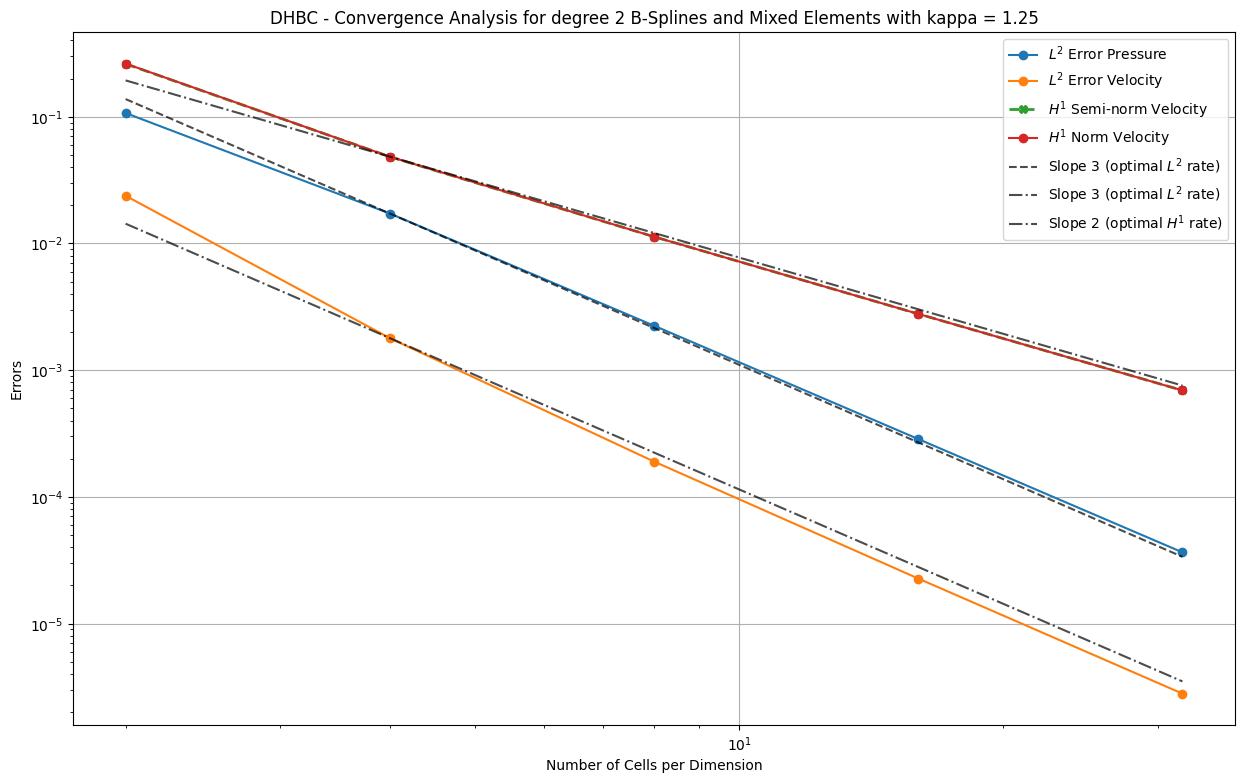
\includegraphics[width=\textwidth]{convergence_degree_2_mixed_dirichlet_homogeneous_kappa=1.25}
		\caption{$d=2$}
		\label{fig:convergencedegree2mixeddirichlethomogeneouskappa1}
	\end{subfigure}
	\begin{subfigure}[b]{0.49\textwidth}
		\centering
		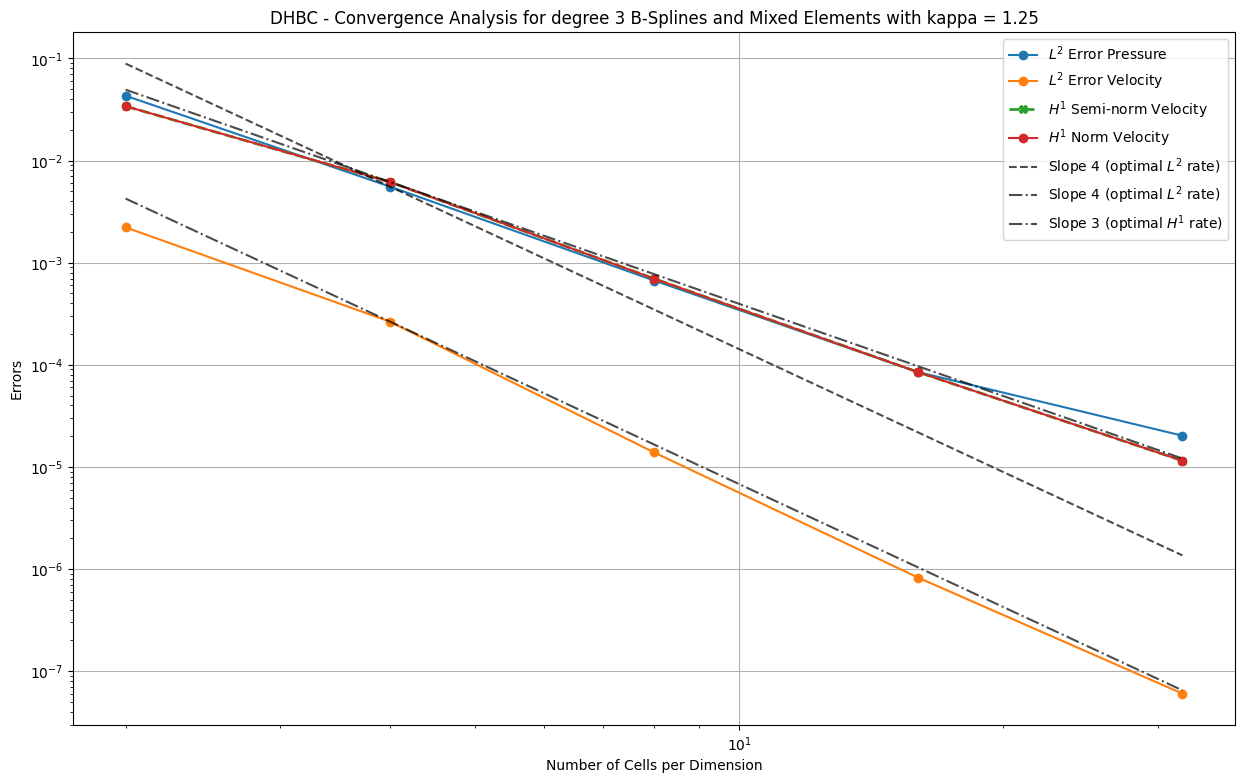
\includegraphics[width=\textwidth]{convergence_degree_3_mixed_dirichlet_homogeneous_kappa=1.25}
		\caption{$d=3$}
		\label{fig:convergencedegree3mixeddirichlethomogeneouskappa1}
	\end{subfigure}
	\\
	\begin{subfigure}[b]{0.49\textwidth}
		\centering
		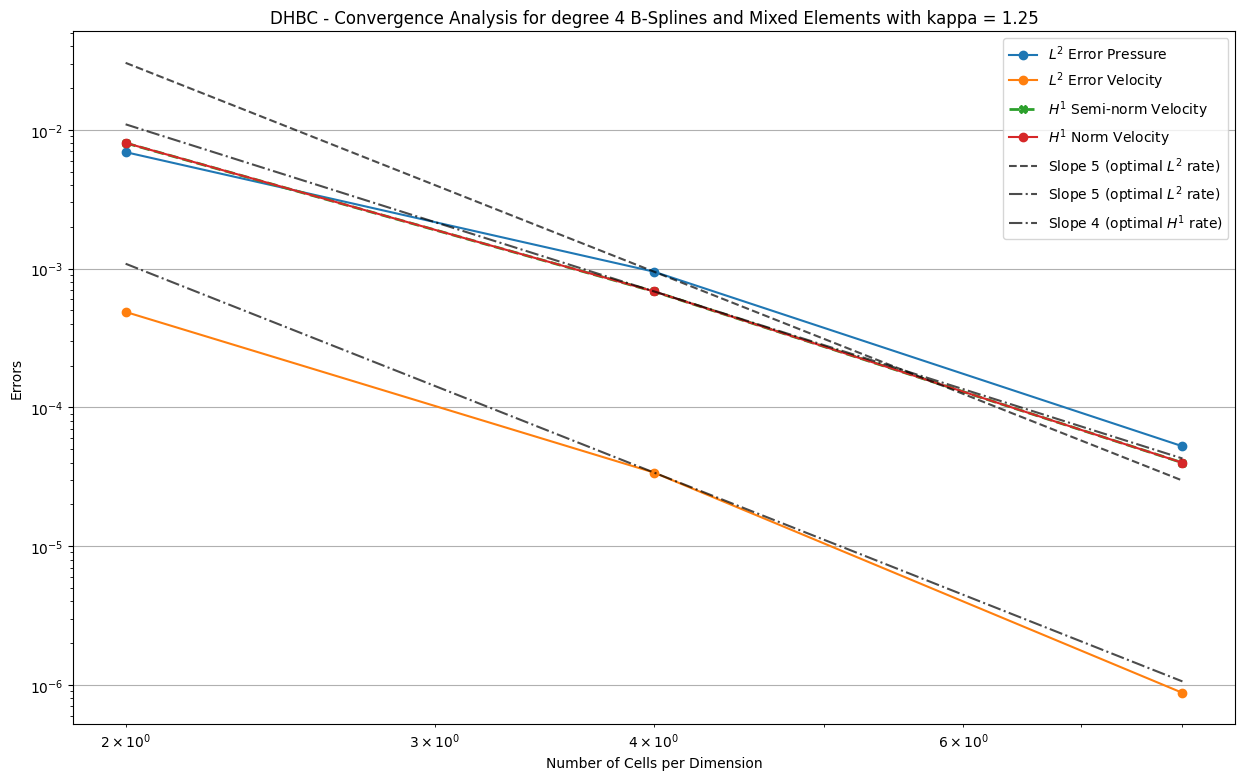
\includegraphics[width=\textwidth]{convergence_degree_4_mixed_dirichlet_homogeneous_kappa=1.25}
		\caption{$d=4$}
		\label{fig:convergencedegree4mixeddirichlethomogeneouskappa1}
	\end{subfigure}
	\begin{subfigure}[b]{0.49\textwidth}
		\centering
		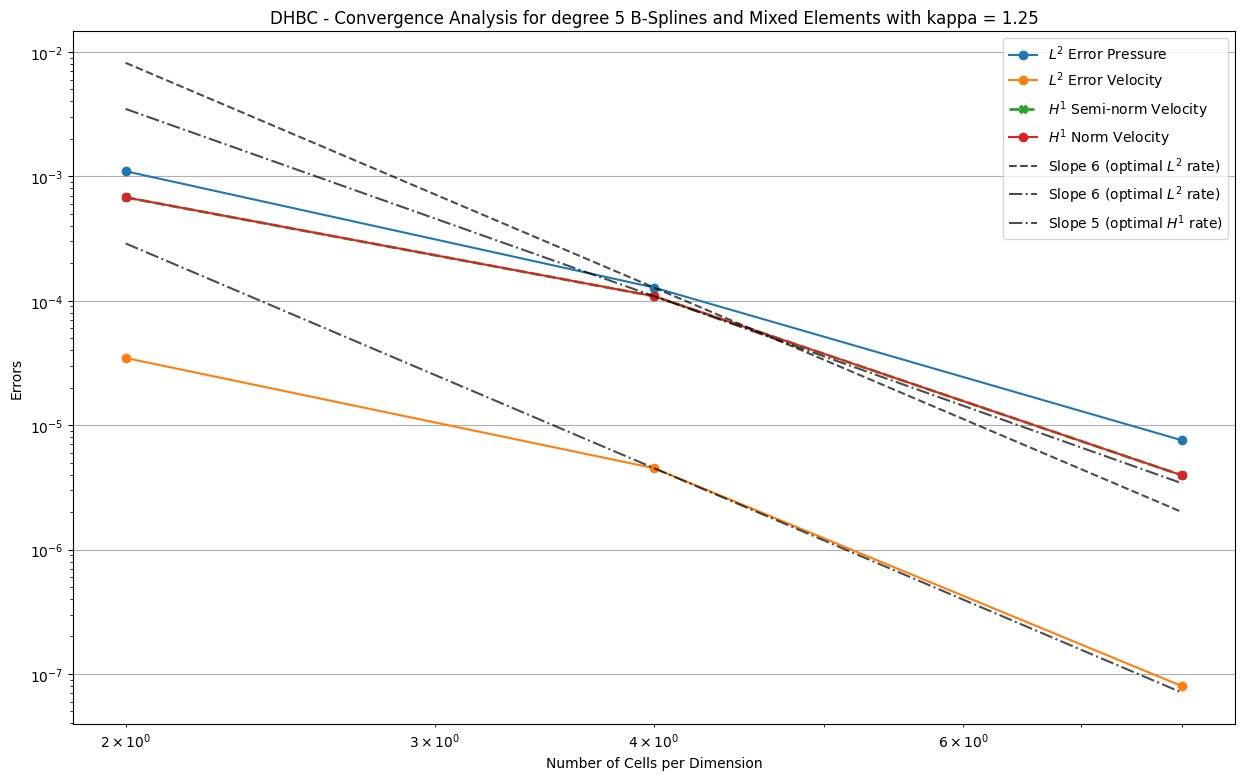
\includegraphics[width=\textwidth]{convergence_degree_5_mixed_dirichlet_homogeneous_kappa=1.25}
		\caption{$d=5$}
		\label{fig:convergencedegree5mixeddirichlethomogeneouskappa1}
	\end{subfigure}
	\caption{Four plots of errors between exact solution and numerical solution with different degree B-Splines (with $\lambda = 1.25$  \& $\mu = 1$) using the mixed formulation}
\end{figure}

\begin{figure}[!h]
	\centering
	\begin{subfigure}[b]{0.49\textwidth}
		\centering
		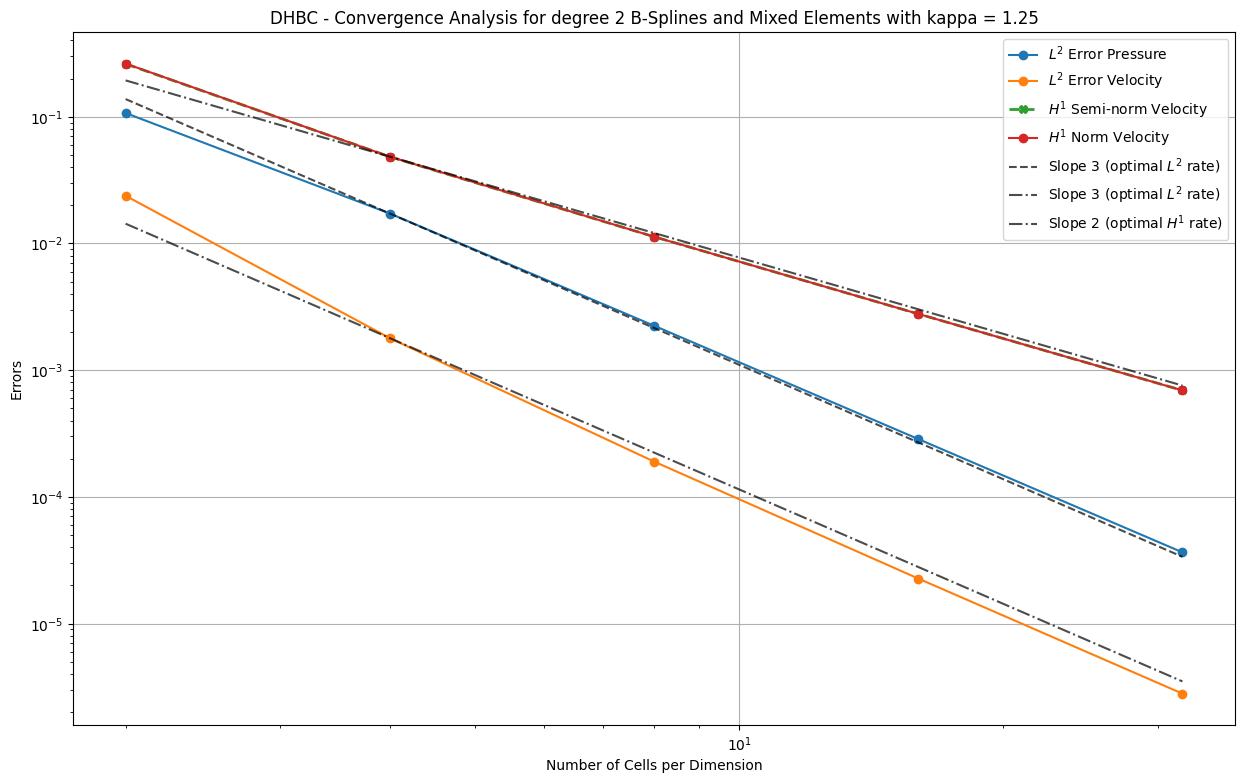
\includegraphics[width=\textwidth]{convergence_degree_2_mixed_dirichlet_homogeneous_kappa=1.25}
		\caption{$\lambda=1.25$}
	\end{subfigure}
	\begin{subfigure}[b]{0.49\textwidth}
		\centering
		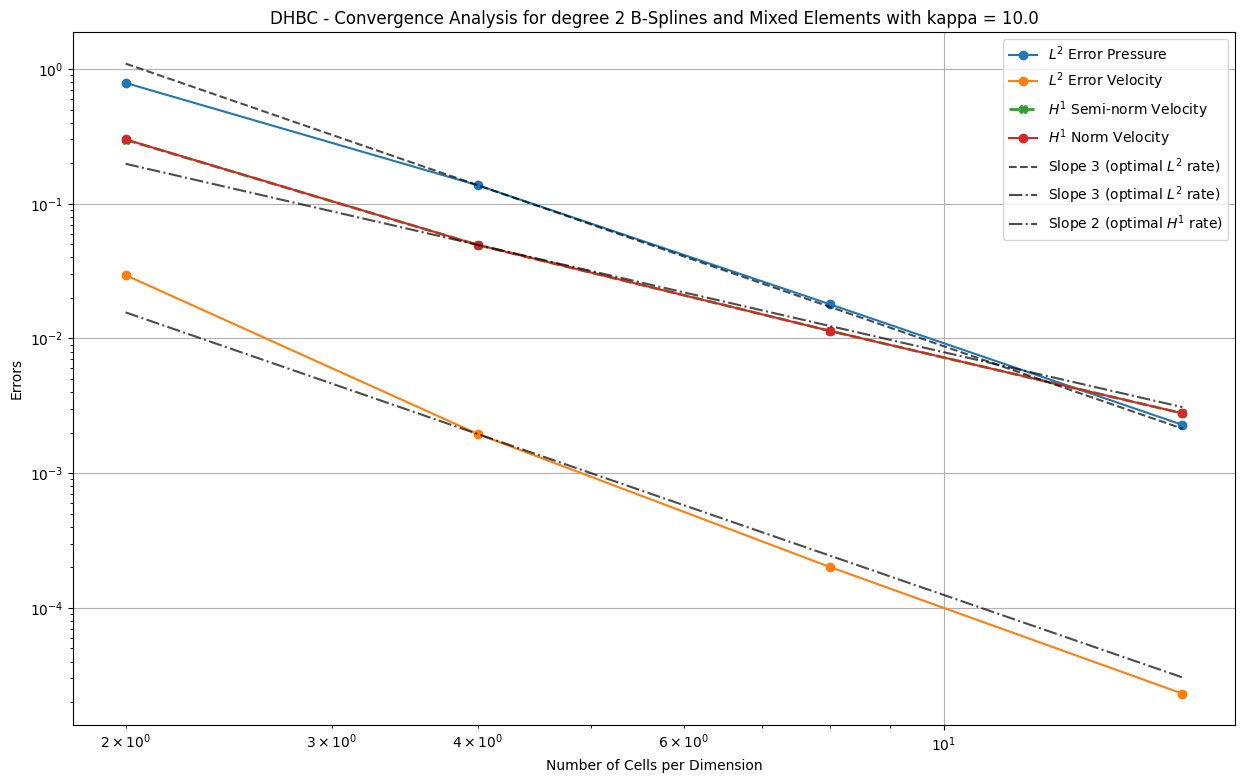
\includegraphics[width=\textwidth]{convergence_degree_2_mixed_dirichlet_homogeneous_kappa=10.0}
		\caption{$\lambda=10$}
	\end{subfigure}
	\\
	\begin{subfigure}[b]{0.49\textwidth}
		\centering
		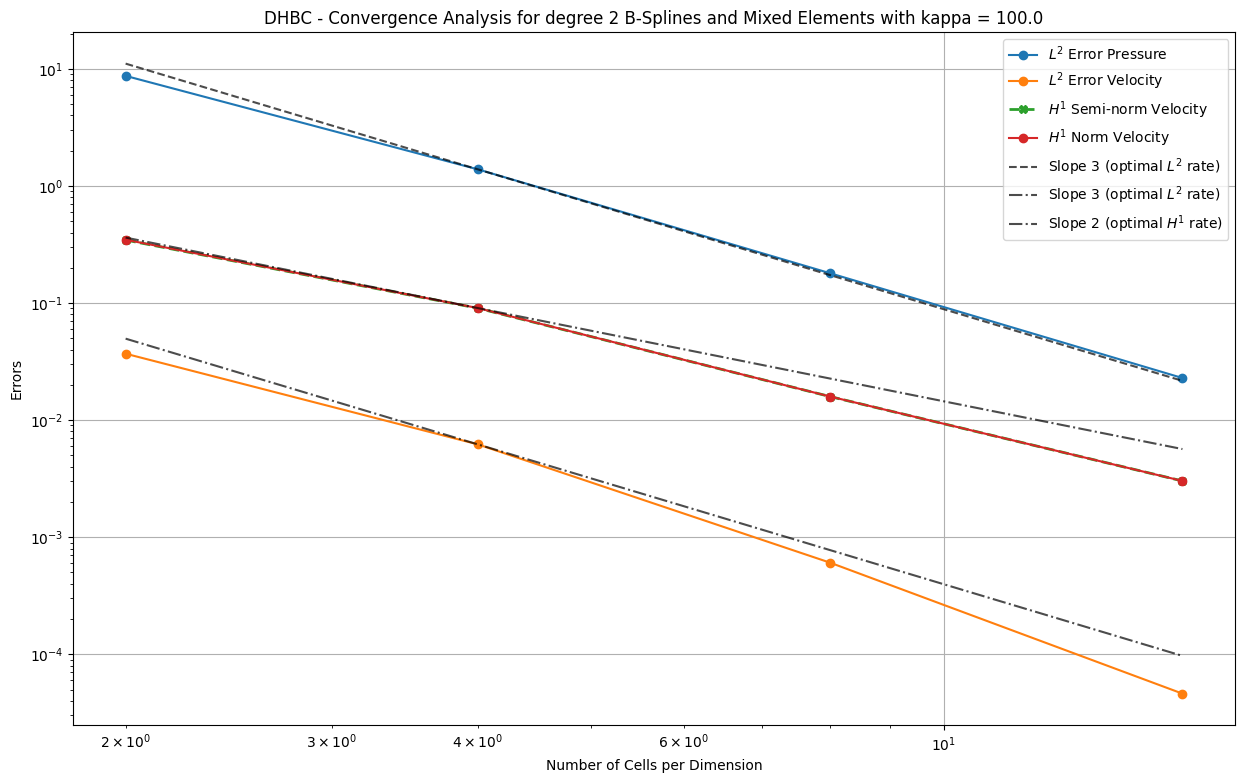
\includegraphics[width=\textwidth]{convergence_degree_2_mixed_dirichlet_homogeneous_kappa=100.0}
		\caption{$\lambda=100$}
	\end{subfigure}
	\begin{subfigure}[b]{0.49\textwidth}
		\centering
		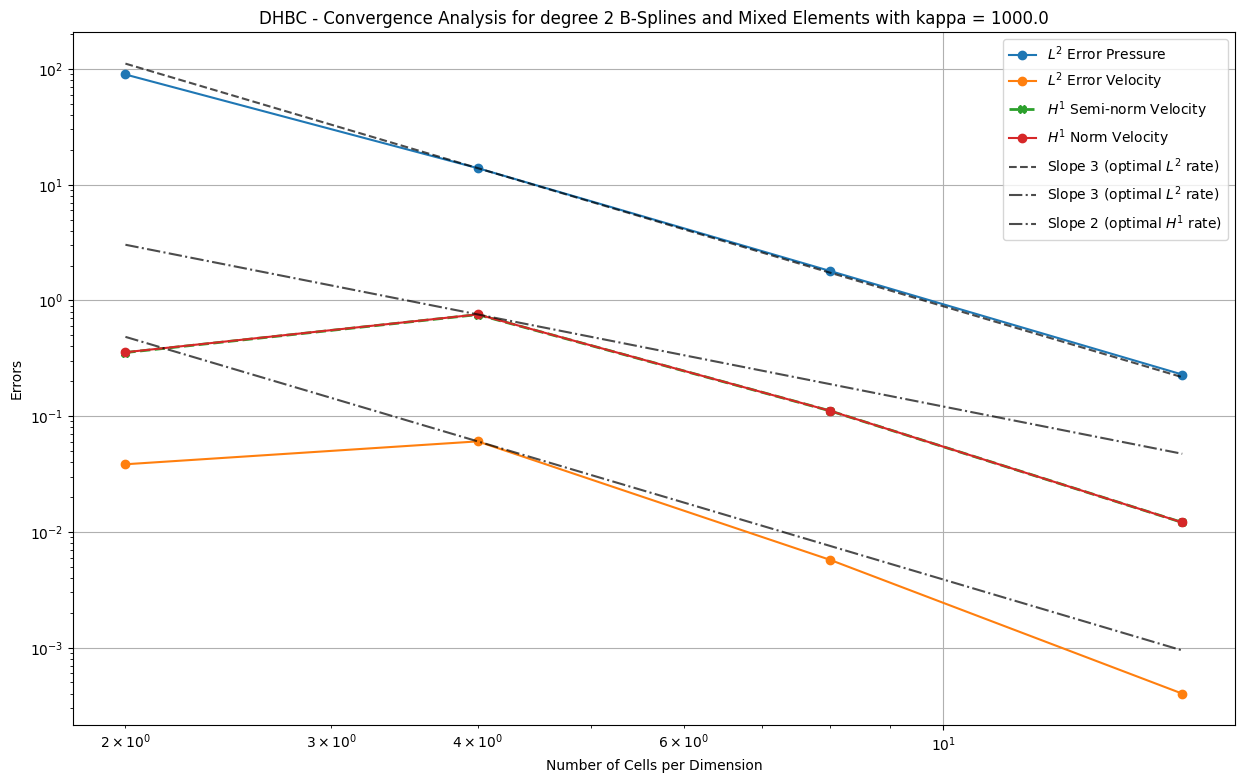
\includegraphics[width=\textwidth]{convergence_degree_2_mixed_dirichlet_homogeneous_kappa=1000.0}
		\caption{$\lambda=1000$}
	\end{subfigure}
	\\
	\begin{subfigure}[b]{0.49\textwidth}
		\centering
		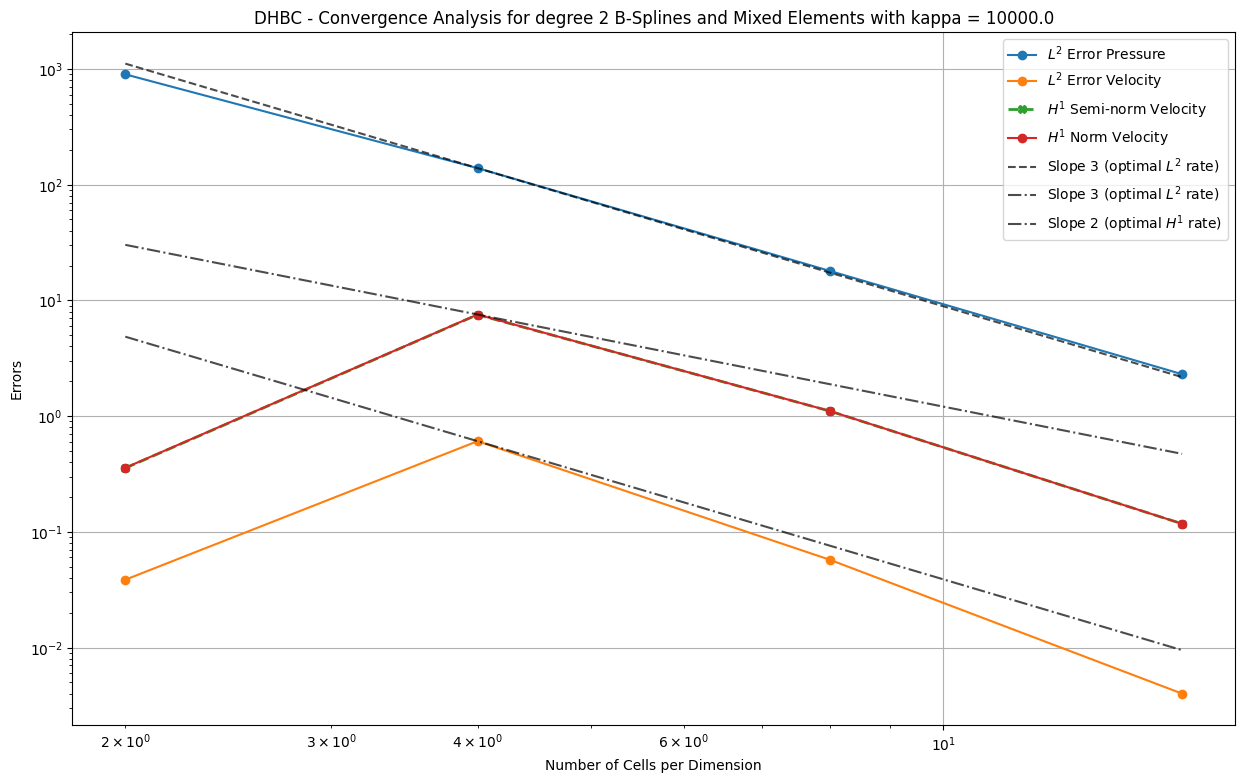
\includegraphics[width=\textwidth]{convergence_degree_2_mixed_dirichlet_homogeneous_kappa=10000.0}
		\caption{$\lambda=10000$}
	\end{subfigure}
	\begin{subfigure}[b]{0.49\textwidth}
		\centering
		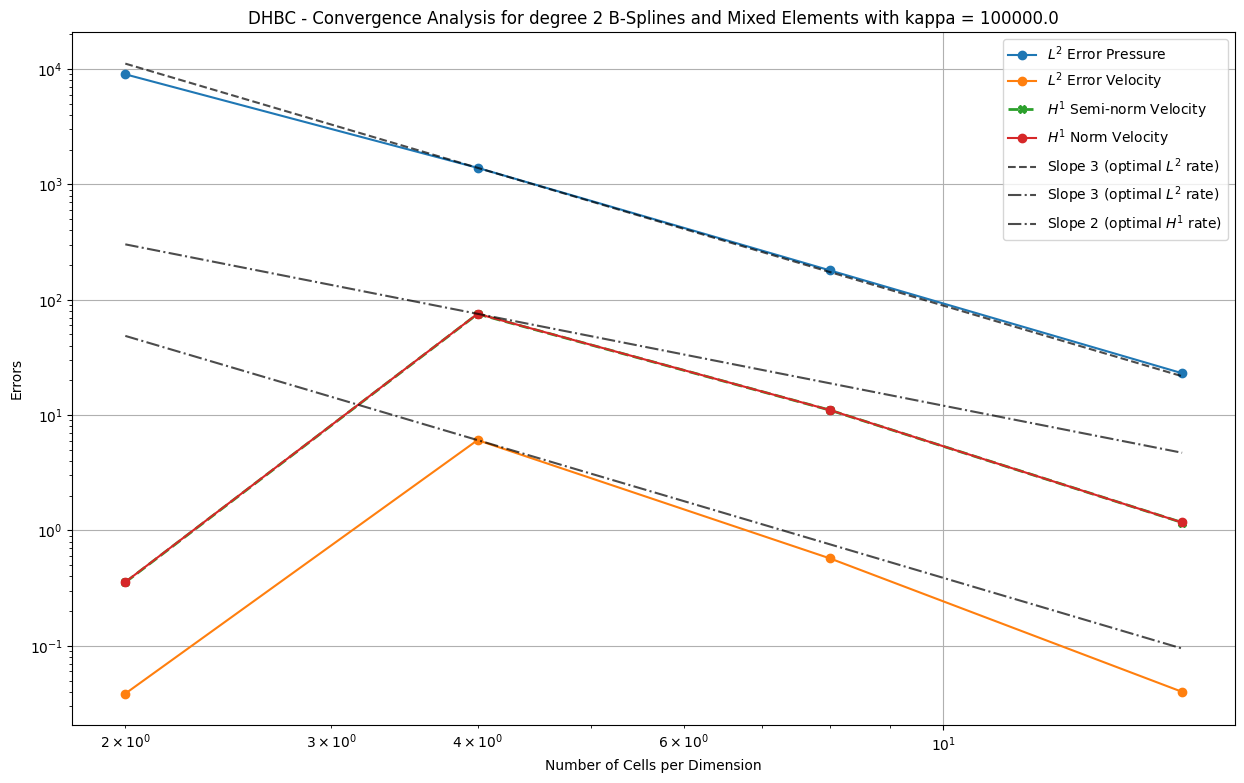
\includegraphics[width=\textwidth]{convergence_degree_2_mixed_dirichlet_homogeneous_kappa=100000.0}
		\caption{$\lambda=100000$}
	\end{subfigure}
	\caption{Error plots between exact solution and numerical solution with degree 2 B-Splines and mixed formulation with increasing values of $\lambda$}
\end{figure}

\newpage
Compare these two formulation in "extreme" cases on the supercomputer ?

\newpage
\printbibliography[heading=bibnumbered]

\newpage
\chapter{Appendices}
\section{Other plots of solutions for the problem with Dirichlet Homogeneous Boundary Conditions}



\end{document}